% NOTES
% https://www.elsevier.com/journals/journal-of-cleaner-production/0959-6526/guide-for-authors
% Original article: Standard research papers of 6000-8000 words in length, with tables, illustrations and references, in which hypotheses are tested and results reported.
% Limit 20000 Characters	

% We might have to or should add a Data in Brief: https://www.elsevier.com/journals/data-in-brief/2352-3409/guide-for-authors

% Math formulae
% Please submit math equations as editable text and not as images. Present simple formulae in line with normal text where possible and use the solidus (/) instead of a horizontal line for small fractional terms, e.g., X/Y. In principle, variables are to be presented in italics. Powers of e are often more conveniently denoted by exp. Number consecutively any equations that have to be displayed separately from the text (if referred to explicitly in the text).

\documentclass[review]{elsarticle}

\usepackage{epstopdf}
\usepackage{lineno,hyperref}
\usepackage{booktabs}
\usepackage{float}
\usepackage{amsmath}
\usepackage{siunitx}
\usepackage{textcomp}
\usepackage{eurosym}
\modulolinenumbers[5]

\renewcommand*{\sectionautorefname}{Section}
\renewcommand*{\figureautorefname}{Figure}
\renewcommand*{\tableautorefname}{Table}
\renewcommand*{\equationautorefname}{Eq.}

\journal{Journal of Cleaner Production}

%%%%%%%%%%%%%%%%%%%%%%%
%% Elsevier bibliography styles
%%%%%%%%%%%%%%%%%%%%%%%
%% To change the style, put a % in front of the second line of the current style and
%% remove the % from the second line of the style you would like to use.
%%%%%%%%%%%%%%%%%%%%%%%

%% Numbered
%\bibliographystyle{model1-num-names}

%% Numbered without titles
%\bibliographystyle{model1a-num-names}

%% Harvard
%\bibliographystyle{model2-names.bst}\biboptions{authoryear}

%% Vancouver numbered
%\usepackage{numcompress}\bibliographystyle{model3-num-names}

%% Vancouver name/year
%\usepackage{numcompress}\bibliographystyle{model4-names}\biboptions{authoryear}

%% APA style
%\bibliographystyle{model5-names}\biboptions{authoryear}

%% AMA style
%\usepackage{numcompress}\bibliographystyle{model6-num-names}

%% `Elsevier LaTeX' style
\bibliographystyle{elsarticle-num}
%%%%%%%%%%%%%%%%%%%%%%%

\begin{document}

%%%%%%%%%%%%%%%%%%%%%%%%%%%%%%%%%%%%%%%%%%%%%%%%%%%%%%%%%%%%%%%%%%%%%%%%%%%%%%%%%%%%%
\begin{frontmatter}

\title{Decarbonisation options in the industry sector and conceptual model of industry in an integrated energy system model}

%% Group authors per affiliation:

\author[mymainaddress]{Frauke Wiese\corref{mycorrespondingauthor}}
\cortext[mycorrespondingauthor]{Corresponding author}
\ead{frwi@dtu.dk}

\author[mymainaddress]{Mattia Baldini}

\address[mymainaddress]{DTU Management Engineering, Technical University of Denmark}

%%%%%%%%%%%%%%%%%%%%%%%%%%%%%%%%%%%%%%%%%%%%%%%%%%%%%%%%%%%%%%%%%%%%%%%%%%%%%%%%%%%%%
\begin{abstract}
% A concise and factual abstract is required. The abstract should state briefly the purpose of the research, the principal results and major conclusions. An abstract is often presented separately from the article, so it must be able to stand alone. For this reason, References should be avoided, but if essential, then cite the author(s) and year(s). Also, non-standard or uncommon abbreviations should be avoided, but if essential they must be defined at their first mention in the abstract itself.



Main question:
\begin{itemize}
    \item \textbf{Should be rather present a conceptual model how to integrate industry in an integrated energy system model OR} 
    \item should we rather do some calculations without the model based on the numbers we have and describe these?
    \item Maybe we can combine it by backing up the model (deriving the model from ) the data and structure of data we prepared for Denmark, then a result can be the features the model needs to have and the main rough numbers which need to be checked by a model having the features of the conceptual model.
    \item What is the fuel switch options to which cost: Maybe we should have a table with the sectors and end-uses their options to decarbonize. This we can already derive without the model runs
\end{itemize}

\end{abstract}
%%%%%%%%%%%%%%%%%%%%%%%%%%%%%%%%%%%%%%%%%%%%%%%%%%%%%%%%%%%%%%%%%%%%%%%%%%%%%%%%%%%%%

\begin{keyword}
% Immediately after the abstract, provide a maximum of 6 keywords, using American spelling and avoiding general and plural terms and multiple concepts (avoid, for example, 'and', 'of'). Be sparing with abbreviations: only abbreviations firmly established in the field may be eligible. These keywords will be used for indexing purposes.
industry decarbonization \sep energy savings\sep fuel substitution \sep electrification\sep integrated energy system model Balmorel \sep process heat
\end{keyword}

\end{frontmatter}
%%%%%%%%%%%%%%%%%%%%%%%%%%%%%%%%%%%%%%%%%%%%%%%%%%%%%%%%%%%%%%%%%%%%%%%%%%%%%%%%%%%%%

\linenumbers

%%%%%%%%%%%%%%%%%%%%%%%%%%%%%%%%%%%%%%%%%%%%%%%%%%%%%%%%%%%%%%%%%%%%%%%%%%%%%%%%%%%%%

\section{Introduction}

In light of the recent Paris Agreement, the necessity to aim at carbon neutral societies and switch to 100\% renewable energy systems is a clear goal. 
As many of the past international protocols, the summit in Paris highlighted the importance to decarbonise energy intensive sectors, reducing greenhouse gas (GHG) emissions. 
In Europe, similar to other countries, two sectors stand out for substantial energy consumption and GHG emissions: power and industry. 
The power sector is historically associated with great use of energy resources because of the nature of most of the energy conversion processes (e.g combustion of fossil fuels). In the last years, the energy sector has been subject to changes with regard to the sources to produce energy. More technologies, based on renewable energy resources, are gradually replacing fossil fuels-based plants. The increasing share of clean technologies in the power mix, along with other interventions (e.g. energy efficiency or sustainable fuels), has been (and is still) reducing the level of GHG emission associated with the power sector.

Likewise, the industry sector starts and is required to follow a similar pathway. 
With more than 125 TWh of electricity consumption, 851 TWh of fossil fuels used for energetic purposes and 671 TWh of fossil fuels feedstock, the industry sector accounted for almost 30\% of the total EU energy consumption in 2010; the related GHGs corresponded to 9\% of the total EU28 emissions stock \cite{Eurostat2017,Lechtenbohmer2016}.
As for the power sector, technical options are available to decarbonise industry. The three main established categories are (i) electrification, (ii) fuel substitution and (iii) improved energy efficiency \cite{Lechtenbohmer2016, Akashi2011, IRENA2014}.

%ELECTRIFICATION
Given the increasing share of renewable energy technologies in the energy systems, electrified processes powered by renewable electricity are expected to replace both fossil fuels used as energy and as feedstock in the near future \cite{Lechtenbohmer2015, EnergyCommission2017, Energikommissionen2017, Lin2017}. \cite{Lechtenbohmer2016} have estimated that, in a simulated 2050 scenario, a deep decarbonisation via electrification of the industry can lead up to almost 300 Mt of $CO_2$ direct savings for the EU28. Also, \cite{IRENA2014} projects a future increase of the share of electricity use in the industrial sector from about 10\%-15\% in 1980s, to 25\%-30\% by 2030 of the total energy consumption.

%FUEL SUBSTITUTION
Fuel substitution is also widely considered for future scenarios \cite{Lin2016,Rehfeldt2016}. \cite{Iea2012} considers that switching fuels and feedstock to renewable fuels (e.g. biogas or hydrogen) can account for 300 $MtCO_2$-eq of emission reduction even in a 4 degrees scenario. This number would increase for more ambitious required scenarios. Similar analyses performed in Italy \cite{Enea2016} and England \cite{Pye2015}, report fuel switch as a main pillar for the transition to a decarbonised energy future.

%ENERGY EFFICIENCY
Furthermore, although studies have acknowledged that the industrial energy efficiency is generally increasing for most of the processes, there is still a large unexploited potential, particularly for industries characterised by high-temperature processes. In a Danish context, \cite{Buhler2016} shows that food, paper and chemical industry are more efficient compared to others processes, characterised by high temperatures. Energy efficiency policies in place in different countries, e.g. China \cite{Li2017,Zheng2017,Lin2017a,Miao2018,Guo2017}, Italy \cite{MazziottiGomezdeTeran2017}, Austria \cite{Karner2015} or Slovenia \cite{Pusnik2017} have proven to be an effective tool to reduce emission from industrial energy-related use, fostering both technology innovation and emission reduction.

In this context of international industry transformation, Denmark is striving to find solutions to reach the 2020 goals \cite{EnergyCommission2017,Energikommissionen2017}. 
With regard to Denmark, examples show that use of heat waste \cite{Buhler2017a}, electrification \cite{DanishEnergyAgency2014a} and adoption of energy efficiency interventions in the industry sector \cite{DEAeff18,Buhler2016} can lower the use of fossil fuels and related GHG emissions. Furthermore, considering recent developments of generation in Denmark, renewable gases have the potential to replace natural gas to some extent \cite{Lise2017,Jensen2017}.
Although these studies indicate promising possibilities, none of the investigations considered the system-wide context of changes of energy supply in the industry sector. 
As both the power and the industry sector are highly interrelated, applying decarbonisation measures in one sector can result in an impact on the other. 
An energy system view/analysis, employing suitable tools like TIMES \cite{IEA-ETSAP}, EnergyPlan \cite{DepartmentofDevelopmentandPlanning} or Balmorel \cite{Wiese2018, balmorel} is thus necessary to assess the size and the scale of these interdependencies.

Although industry covers a relevant share of energy usage, the industrial sector is rather under-represented in most energy system models, particularly when investigating scenarios on decarbonisation pathways.

For the exploration of industrial decarbonisation options enforcement and the related transformation of the Danish energy system, a detailed model of the industry sector is required. It should not only consider the structure of the processes with regard to input fuels, temperature heat levels and fuel use characteristics, but also temporal profiles and geographical location of energy consumption.

The goal of the paper is thus threefold: 1) provide a representation of the Danish industry characteristics highlighting the potential for decarbonisation options, 2) propose a method to model the industrial sector, with fairly high level of detail, within an energy system model and 3) present preliminary results of applying decarbonisation options in the Danish energy system.

By means of the Danish case study, we can assess the influence of modelling the industry sector at higher level of detail in an energy system model and analyse results for future and decarbonised energy system configurations. 

The remainder of the paper is structured as follows: \autoref{inddescr} provides an insight on the Danish industry sector, \autoref{meths} presents the methods adopted and \autoref{datadescr} describes the input data and its processing used for the study. \autoref{outcdisc} reports the empirical results and provides a discussion on the outcomes and \autoref{endofpaper} concludes the paper highlighting the relevant findings and suggests future research.
%%%%%%%%%%%%%%%%%%%%%%%%%%%%%%%%%%%%%%%%%%%%%%%%%%%%%%%%%%%%%%%%%%%%%%%%%%%%%%%%%%%%%

\section{Characteristics of the Danish industry sector} \label{inddescr}

\subsection{Structure of the Danish Industry}
This section provides a description of the elements characterising the Danish industrial sector.

In the literature, industry is the term that commonly refers to a diverse variety of processes characterised by high energy intensity and use. As the term does not have a standard definition, the processes considered to represent the industrial sector vary from study to study, making similar analyses on the field difficult to compare. \cite{Buhler2016} shows that, compared to other studies which considered a restricted number of processes and industries \cite{Oladiran2007,Al-Ghandoor2010,Dincer2003,Sanaei2012}, the results derived from a broader approach provide additional insights and a stronger reliability. In this study, we will thus include agriculture, manufacturing and services in the term \textit{industry} and \textit{industry sector}. In this study we do not consider transportation, neither as sector, nor as end-use within the industry sector. 

\cite{VM2015} have analysed the energy use in Danish industry in a high level of detail. They provide the yearly energy demand of 57 different sectors for 20 types of fuel and 22 types of end-use for the year 2012. The distribution of fuels amongst the process categories is also provided. As refinery, public service and construction are not included in the list of sectors for which detailed end-use data is provided \cite{VM2015}, they will not be included in this study.

%The 22 energy end-uses can be clustered in four groups: \textit{internal conversion losses}, \textit{process heating} (heating/boiling, drying, inspissation, distillation, burning/sintering, melting/casting, other process heating up to/over 150 C), \textit{space heating} and \textit{utilities} (energy for heat pumps, lightning, pumping, comfort cooling, cooling/freezing, comfort ventilation, blowers, compressed air, hydraulic machinery, other electric motors, IT and electronics, other electric consumption).
%\\
%Twenty fuel types supplying processes include coal, fuel oil, petroleum coke, coke, diesel, gasoline (unleaded and coloured), LPG, natural gas, gas-oil, bio-gas, biomass (wood chips, wood pellets and straw), bio-oil, waste, electricity, district heating, solar heating and heat pumps.
%\\
The 57 industrial sectors are clustered in five groups according to similarities in temporal patterns of energy consumption: agriculture, production single shift, production double shift, production triple shift and services. The underlying assumptions behind the classification are based on \cite{VM2016,Wiese2017}.

The consumption in agriculture follows a pattern linked to seasonal dependent activities, with lower energy use during summer and higher during fall and winter. Throughout the week, the consumption is higher during the day (working hours from 6 to 18) and week days and lower by night and in the weekend.

For services, the energy consumption is higher during daytime and weekdays, and lower during the nights and weekend, thus representing activities mostly conducted during normal working hours. Over the year, the energy consumption is mostly constant, apart from energy for space heating purposes.

The production group includes manufacturing and extraction processes. The subdivision in single, double and triple shift is linked to the weekly activities. Single shift facilities typically operate during normal working hours in the week days and are closed during weekends/holidays; double shift have longer operating hours (about 15 hours a day), they close during the night and often during weekends/holidays;
triple shift facilities run as continuous production (i.e. almost constant consumption throughout the year) and close down only few times a year. 
Sectors belonging to this group often present a steady base-load consumption for processes such as auxiliaries or ovens. \\

These categories will be used in the following for illustration. Their practicability with regard to time-related data like demand profiles will further be described in \autoref{sec:profiles}.

%%%%%%%%%%%%%%%%%%%%%%%%%%%%%%%%%%%%%%%%%%%%%%
\subsection{Energy use in Danish industry}
\label{sec:energy_use}

Based on the structure described, \autoref{total_use} illustrates the total energy use by fuel for the Danish industry groups for the year 2012.
The industry's energy use accounts for $\sim$156 PJ, distributed between production ($\sim$88 PJ), service ($\sim$48 PJ) and agriculture ($\sim$19 PJ). In the production sector, double ($\sim$44 PJ) and triple shift ($\sim$39 PJ) cover a significant higher share compared to the single shift group ($\sim$5 PJ).

\begin{figure}
\centering
\begin{minipage}{.5\textwidth}
  \centering
  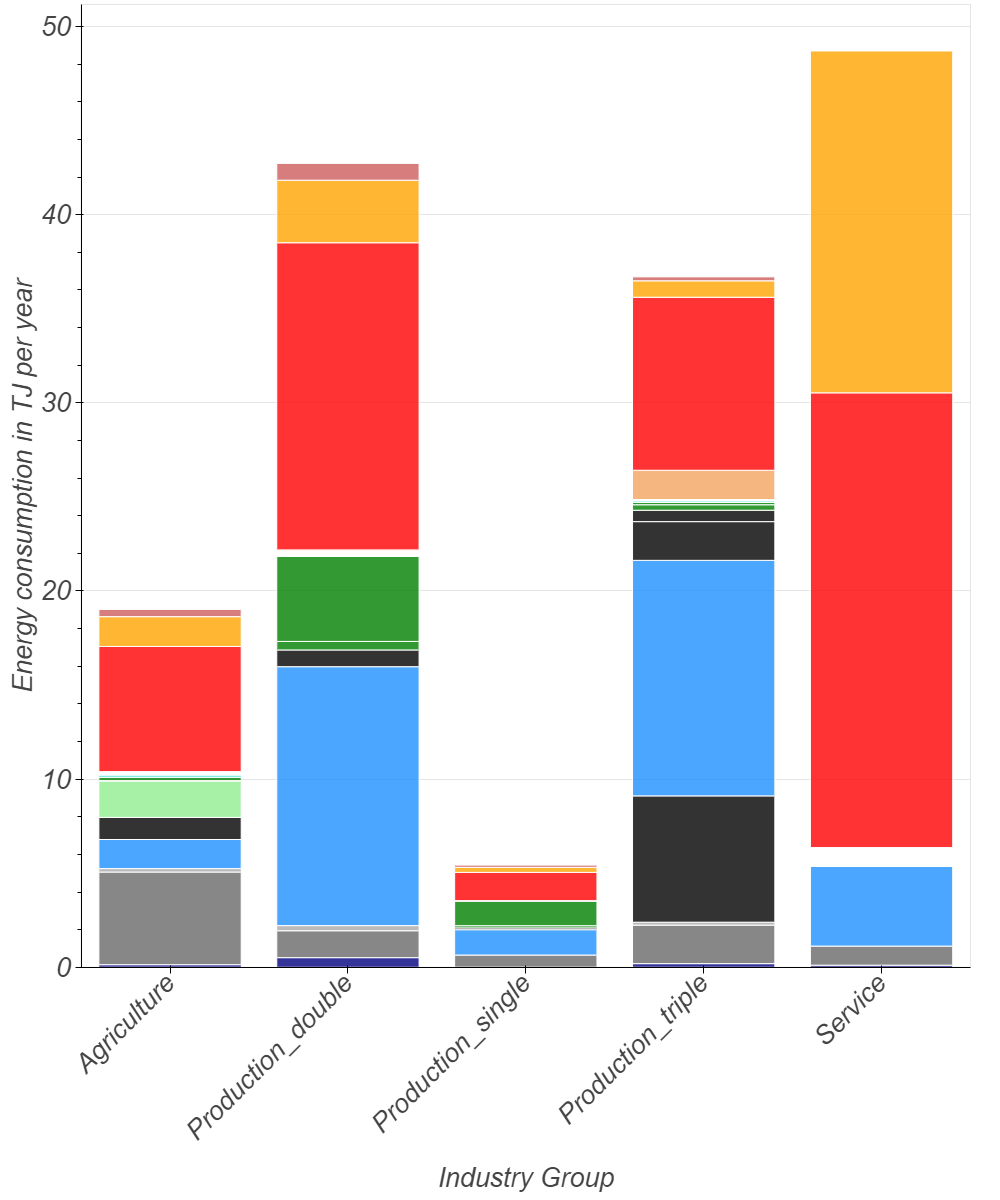
\includegraphics[width=\linewidth]{Img/dan_ind/overview_total.png}
\end{minipage}%
\begin{minipage}{.3\textwidth}
  \centering
  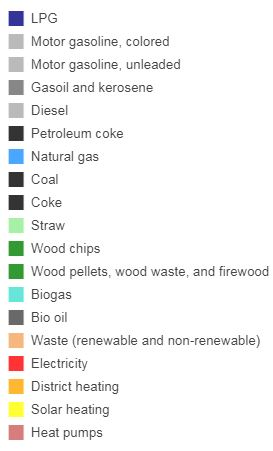
\includegraphics[width=\linewidth]{Img/dan_ind/legend}
\end{minipage}
  \caption{Total energy use in Danish industry groups by fuel \cite{VM2015}}
  \label{total_use} 
\end{figure}

The fuel consumption among the sectors is distributed unevenly, with electricity (36\%), natural gas (21\%), district heating (15\%), gasoil/kerosene (6.4\%) and petroleum coke (4\%) covering the majority of the consumption, while the other fuels contribute to a minor extent.


\iffalse
\autoref{heatmapagri}, \autoref{heatmapprod}, \autoref{heatmapserv} provide an indication on the fuel-use for the different industrial processes. For the production group the data are reported as a single aggregated cluster.

\begin{figure}[H]
\centering
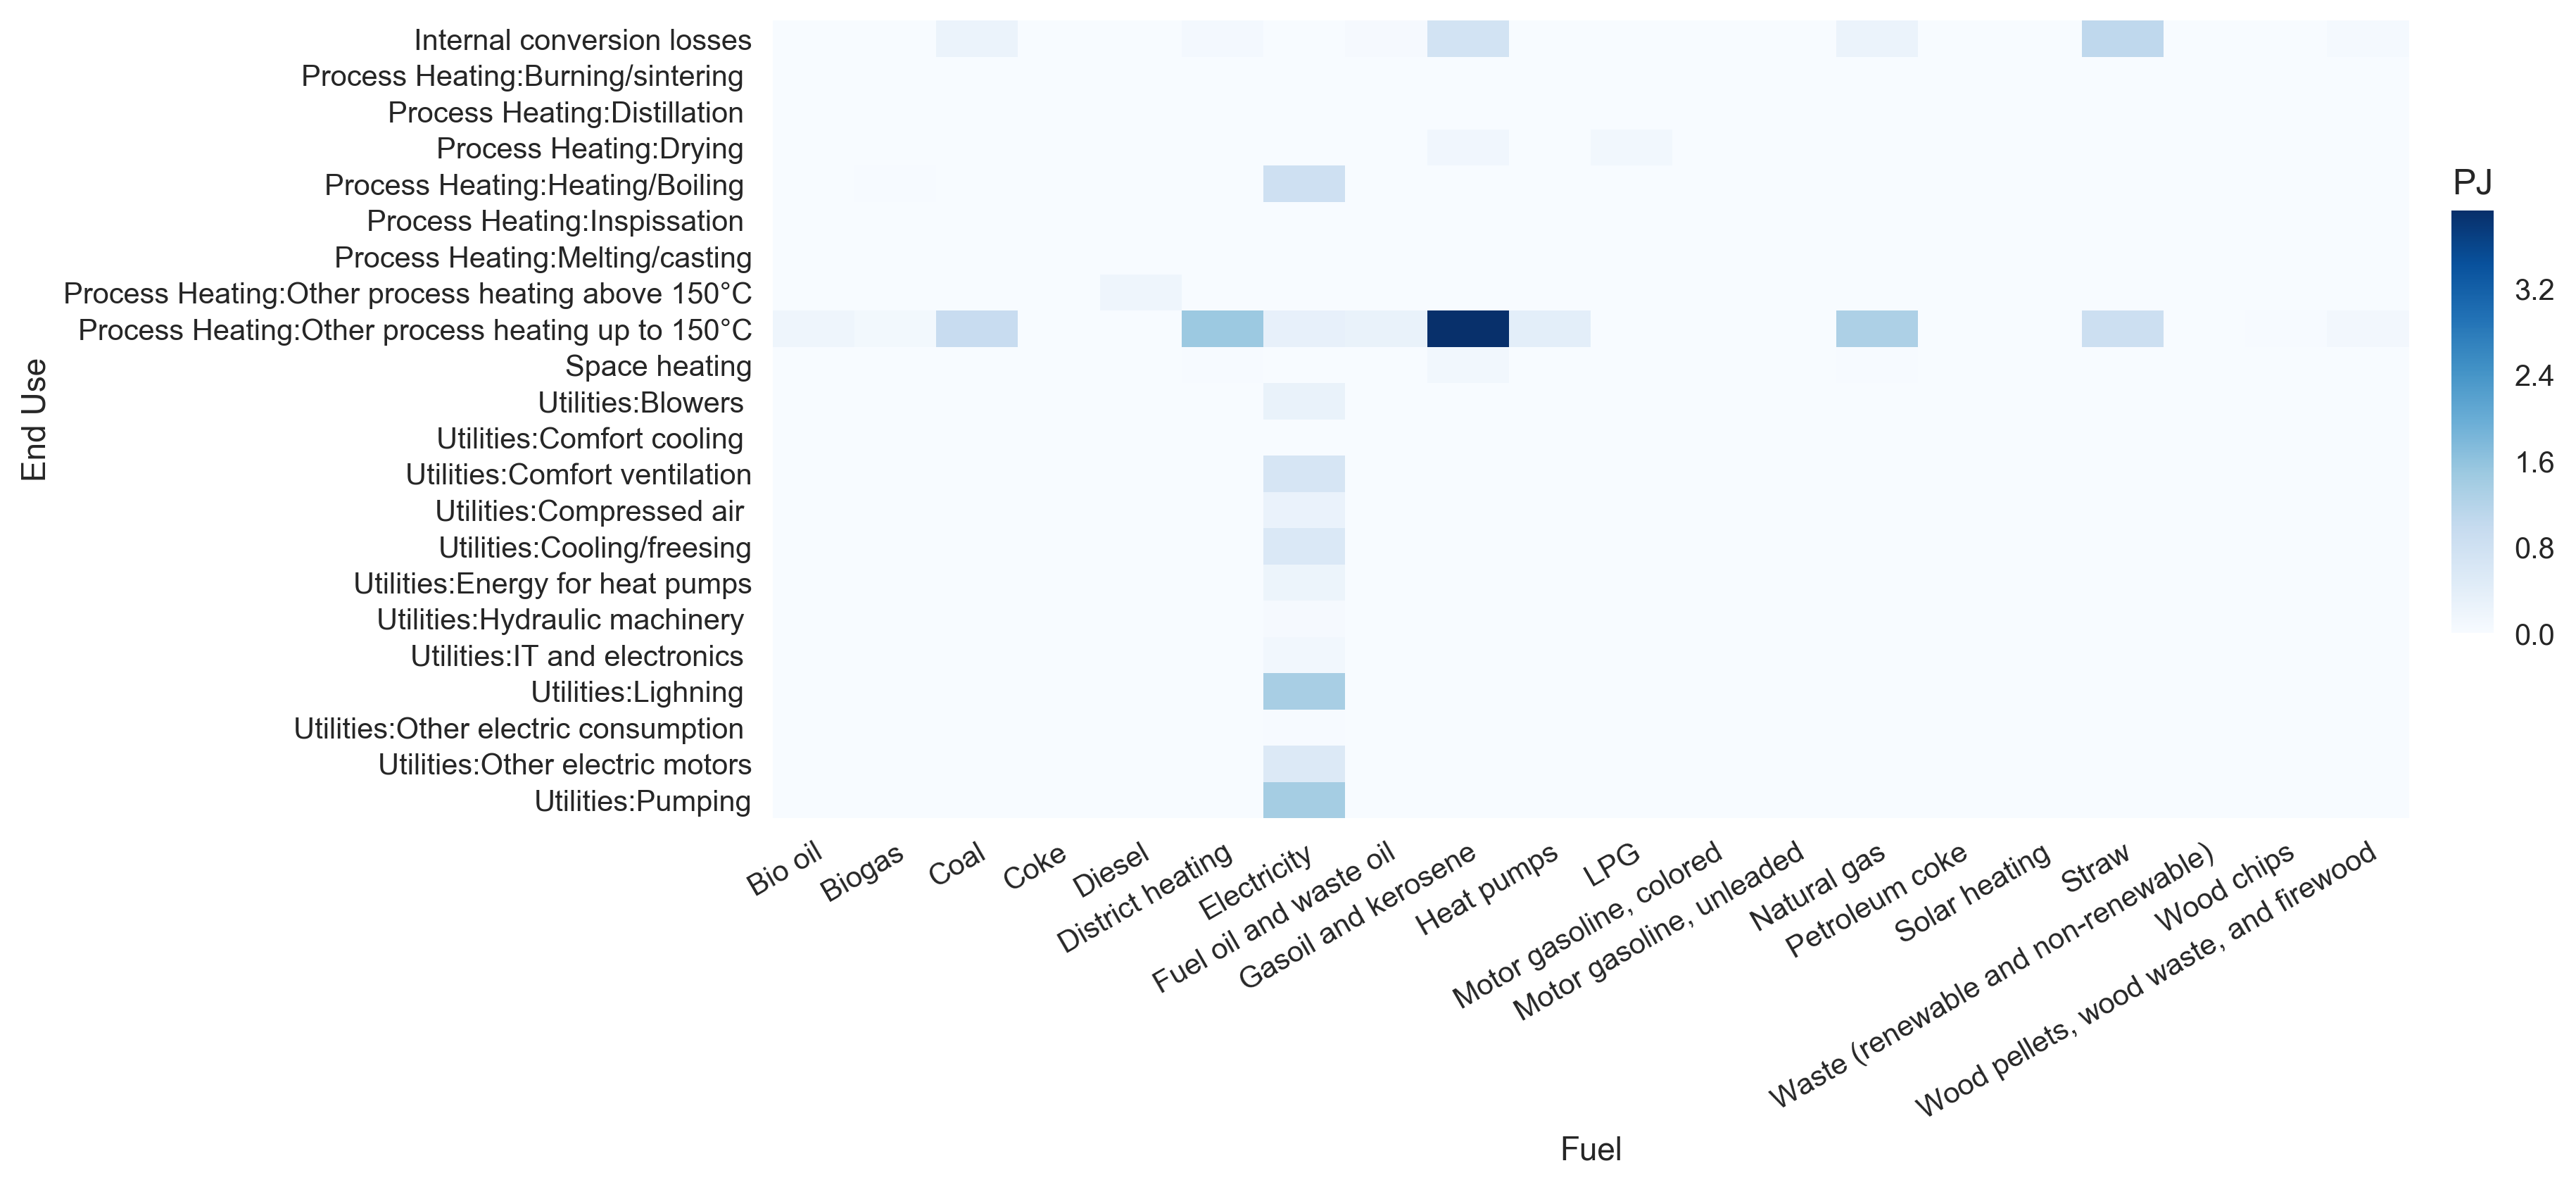
\includegraphics[width=\linewidth]{Img/dan_ind/heatmap_agri.png}
\caption{Breakdown of energy consumption by end-use and fuel in agriculture \cite{VM2015}}
\label{heatmapagri} 
\end{figure}

\begin{figure}[H]
\centering
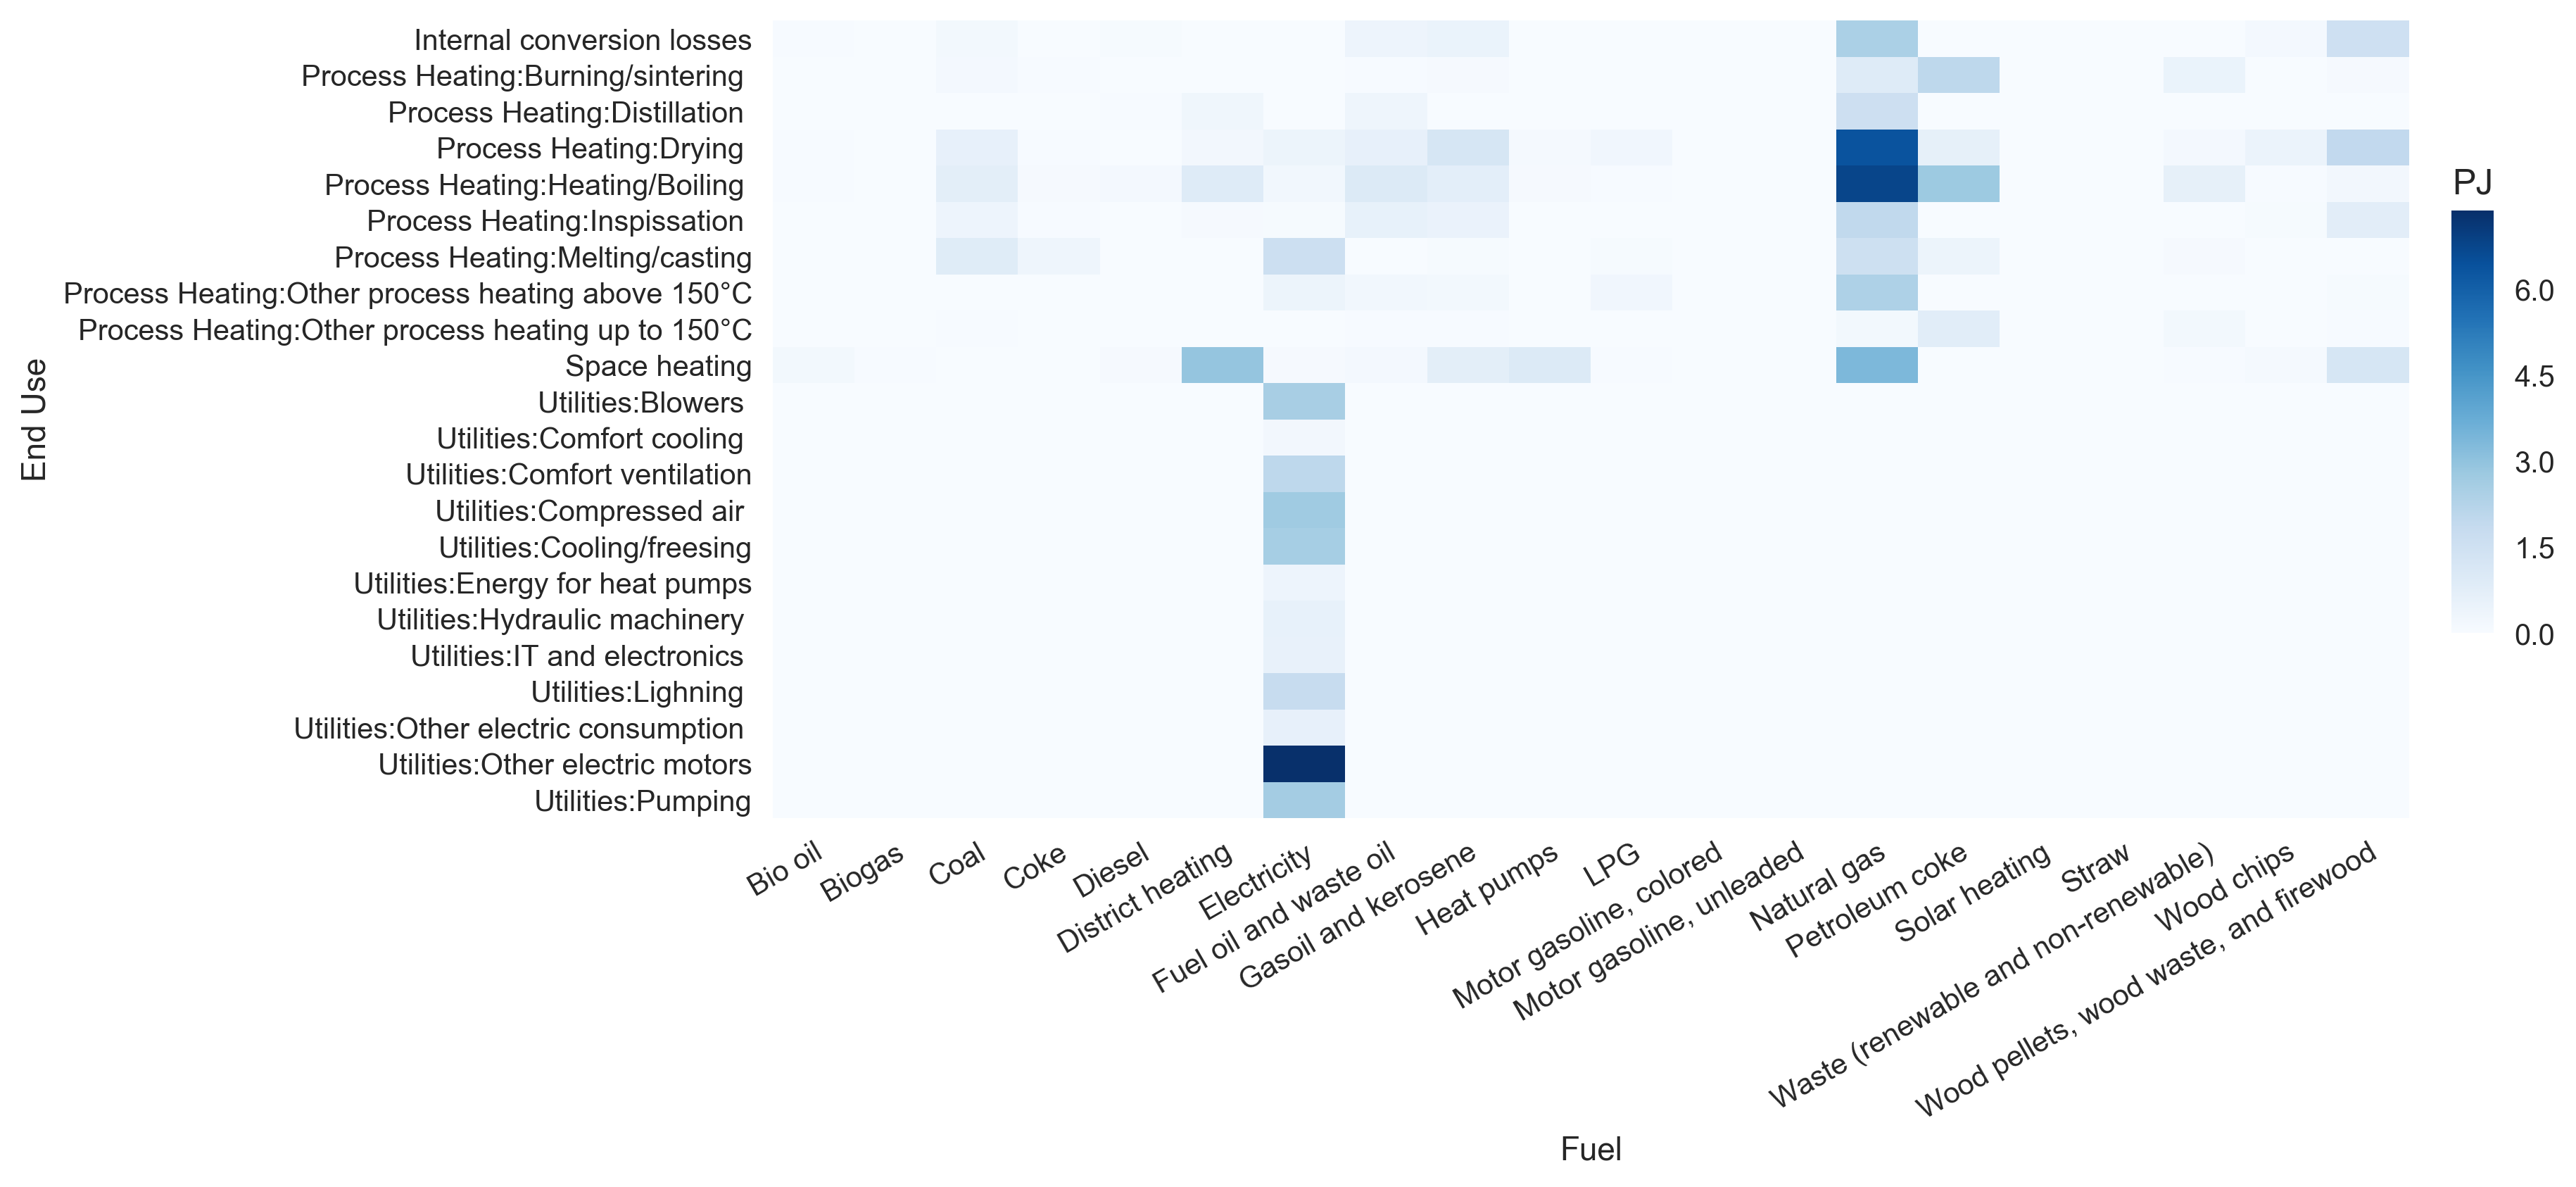
\includegraphics[width=\linewidth]{Img/dan_ind/heatmap_prod.png}
\caption{Breakdown of energy consumption by end-use and fuel in production \cite{VM2015}}
\label{heatmapprod} 
\end{figure}

\begin{figure}[H]
\centering
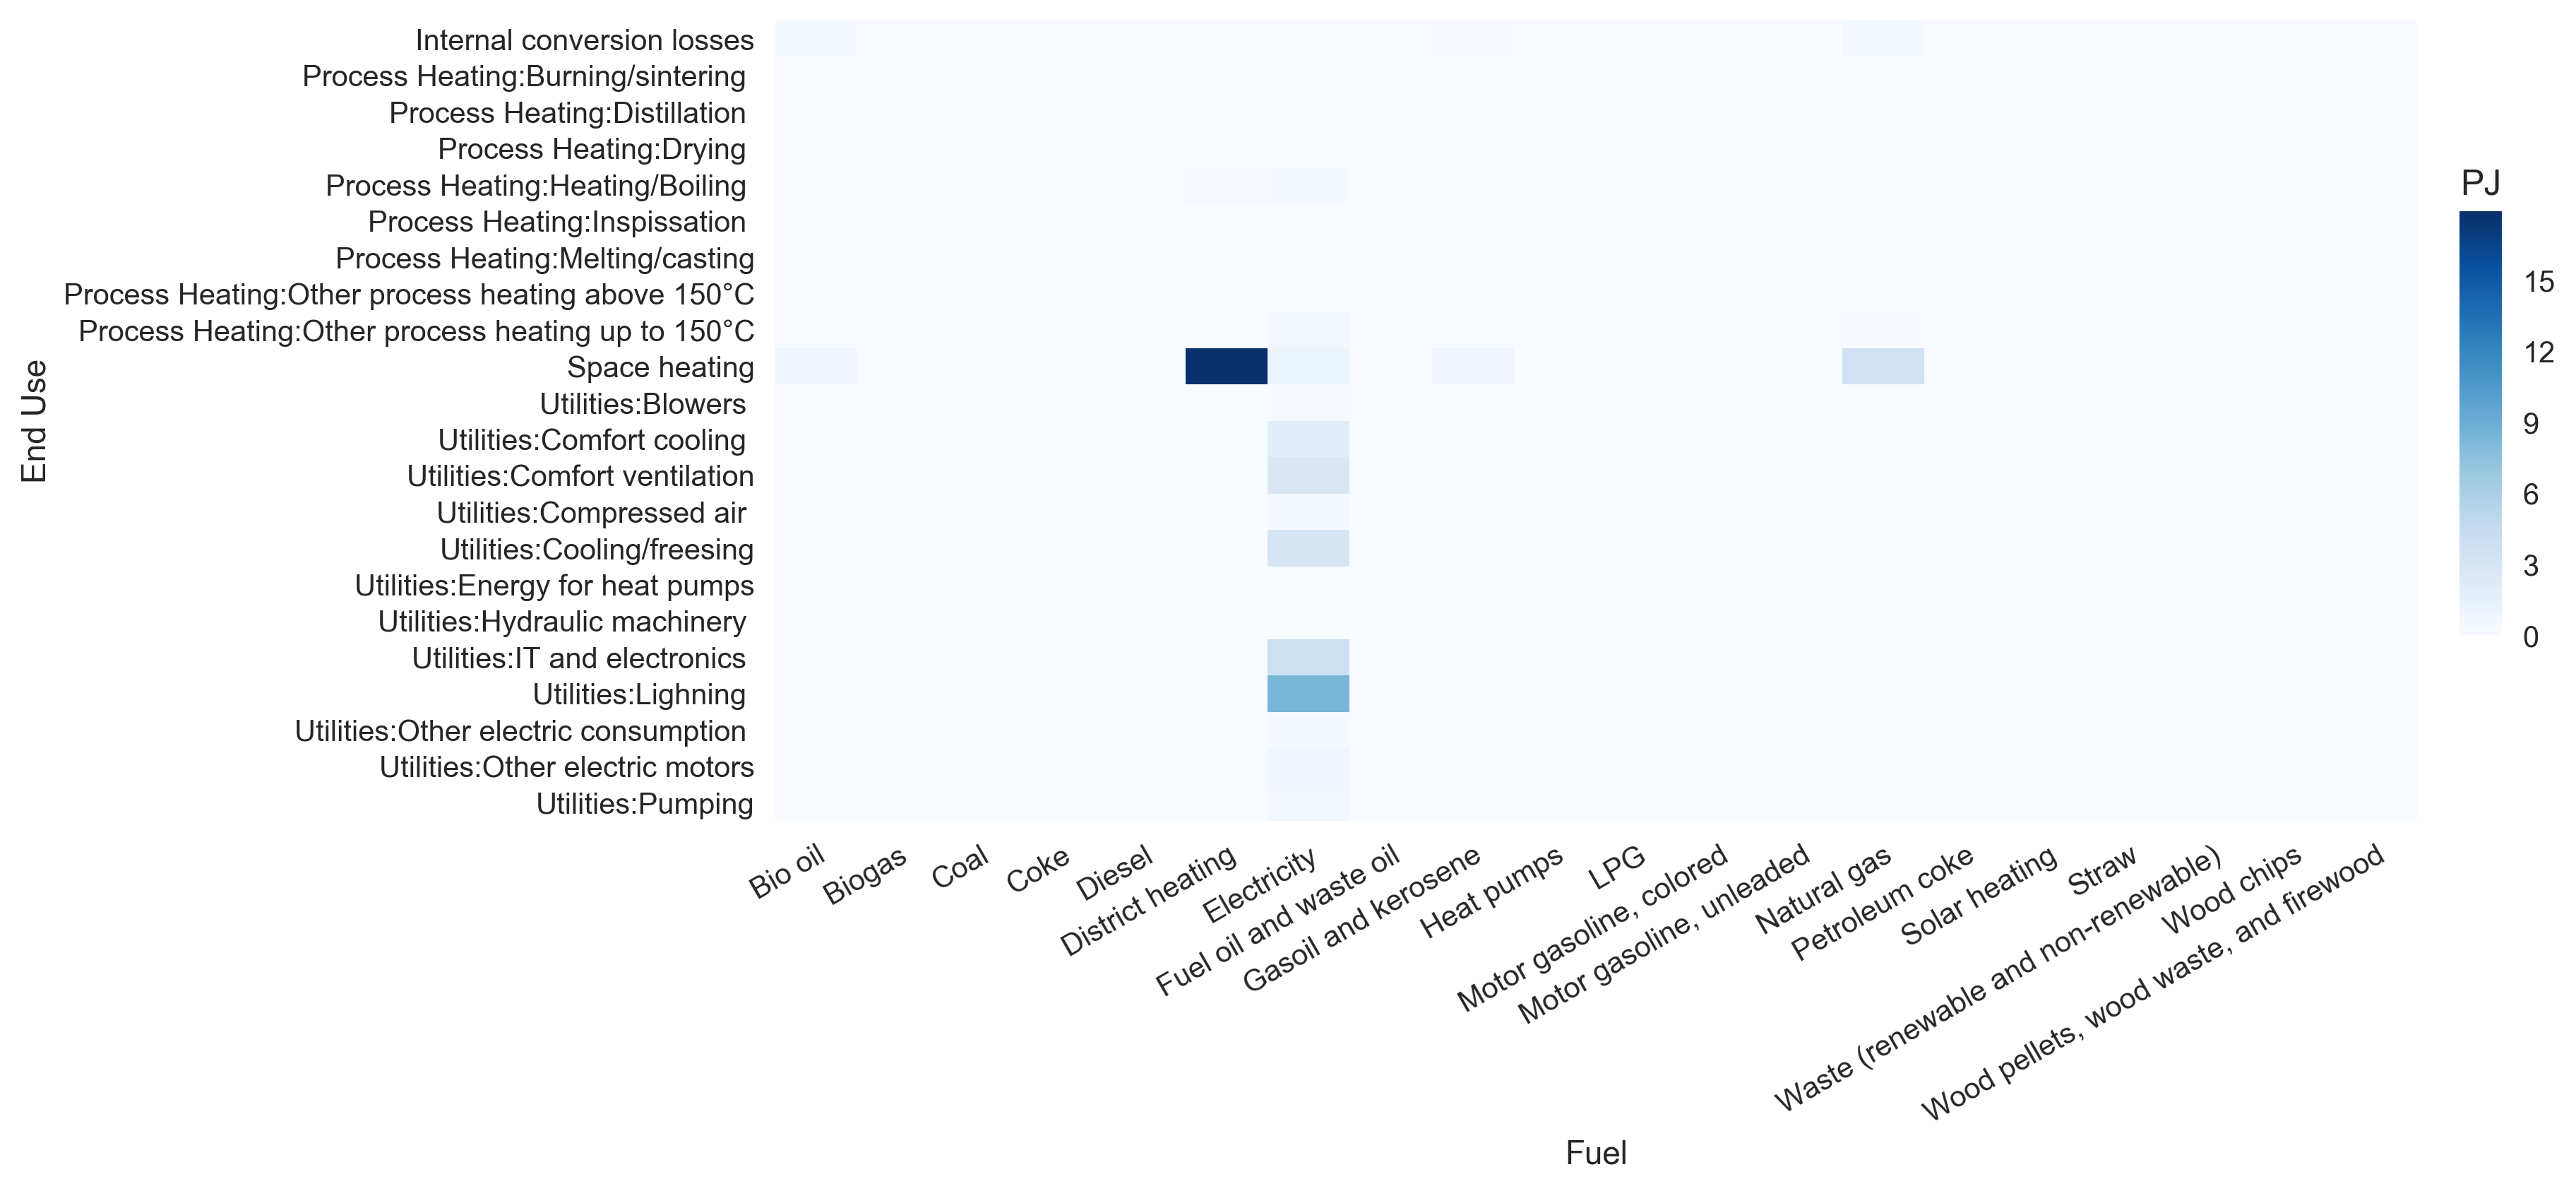
\includegraphics[width=\linewidth]{Img/dan_ind/heatmap_serv.png}
\caption{Breakdown of energy consumption by end-use and fuel in services \cite{VM2015}}
\label{heatmapserv} 
\end{figure}
\fi

The heat maps, presented in three clustered groups, provide a useful indication on the most energy-intensive processes and on the most employed fuels. 
In agriculture, most of the fuel consumption is related to heating up to 150\textdegree (51\%); in production, drying (15\%), heating/boiling (16\%) and space heating (11\%) are predominant; while in service, space heating (50\%) and lightning (17\%) together consume more than half of the total fuels used.

%top up with data
In production, there is a high diversity of end-use; the role of natural gas as a fuel is predominant. 
Space heating and electricity dominate the total energy use in the service sector. District heat is the main fuel supplying space heat, followed by natural gas.

Furthermore, the data show an uneven distribution of fuel consumption in the various groups, with electricity (34\%) and gasoil/kerosene (25\%) being predominant in agriculture, electricity (31\%) and natural gas (31\%) in production, and electricity (50\%) and district heating (37\%) dominating the service sector.

This description of the Danish industry constitutes the bases to model this sector and to investigate its decarbonisation options. With a clear overview of the end-use processes and the related fuel consumption, the industry sector can be conveniently integrated in an energy system model. 
The following section proposes a mathematical model for the industry sector in an integrated energy system model.



%%%%%%%%%%%%%%%%%%%%%%%%%%%%%%%%%%%%%%%%%%%%%%%%%%%%%%%%%%%%%%%%%%%%%%%%%%%%%%%%%%%%%

\section{Methods} \label{meths}

%%%%%%%%%%%%%%%%%%%%%%%%%%%%%%%%%%%%%%%%%%%%%%
\subsection{Balmorel: energy system model}

The application of energy system models facilitates the assessment of the industry's role in achieving pathways to decarbonised energy systems. As commodities like electricity and heat are highly related, in both power and industry sector (e.g. due to the use of heat pumps), only a simultaneous consideration can reflect cost-minimal solutions from a system perspective. This allows to investigate what is defined as "socio-economic welfare maximisation" under different conditions. 
Among the tools available in the literature \cite{Connolly2010}, the energy system model Balmorel is adopted for the analysis \cite{balmorel}.
Balmorel is an open source, mostly linear energy system model that optimises investments and operation of power plants, storage devices and transmission lines for geographical area that can be defined by the user \cite{Ravn2001,Wiese2018}. 
The model considers a set of neighbouring countries operating in an interconnected electricity market. Each country is composed by one or several regions. Electricity can be traded and transmitted between connected regions, with limits imposed by given transmission capacity. 
To consider the heat sector, each electricity region is divided into several district heating areas (DH). Heat transmission among such areas is not allowed.  
\\
Balmorel considers time according to years, seasons (often used as weeks) and individual time units (often used as hours). The user can choose the time horizon and time resolution of the analysis depending on the requirements for the specific investigation.
\\
The model allows to simulate scenarios where demand and supply of electricity and heat are balanced. Operation and investments are optimised, considering local generation vs. import/export, price elasticity of the demand and other characteristics typical for energy systems \cite{Munster2012}. 
\\
The model relies on a set of exogenous input data, including existing capacities of electricity and heat generation technologies, transmissions lines and heat and power demand. 
Energy generating technologies include CHP (both back-pressure and extraction), heat pumps, storage devices (for electricity and heat), and renewable based production technologies (hydro, wind, solar).
Additional key assumptions relate to fuel prices and CO2 costs. Furthermore, taxes and support schemes are required for specific analysis on impacts of different policies.
The data for the model can be chosen for personal application in specific analyses.
\\
The model has been previously applied for a wide range of studies, such as integration of renewable technologies in the energy mix \cite{Ball2007}, analysis of market conditions \cite{Jensen2008}, policies implementation \cite{Karlsson2008}, future role of district heating \cite{Munster2012,Munster2010} and impact of energy efficiency technologies in the energy system  \cite{Baldini2016a}.

The main Balmorel model is supplemented with several addons that allow for specific investigations \cite{Wiese2018}. As a comprehensive representation of the industry sector is not included yet, we propose to enhance the model with details about industrial energy use and different heat levels and their respective replacement options.

%%%%%%%%%%%%%%%%%%%%%%%%%%%%%%%%%%%%%%%%%%%%%%
\subsection{Modelling of the industrial sector}

The energy system model Balmorel considers the industry sector, within the optimisation framework, only as a part of the total heat and electricity consumption. Thus the end-use process specification, previously described, are currently not represented. That means, all fuel and process heat demand not covered by district heat are not accounted for. The black dotted line in \autoref{ensyst} represents the boundaries in the current version of Balmorel, where electricity and district heat demand from industry is considered simply as part of the total energy demand. 

\begin{figure}[H]
\centering
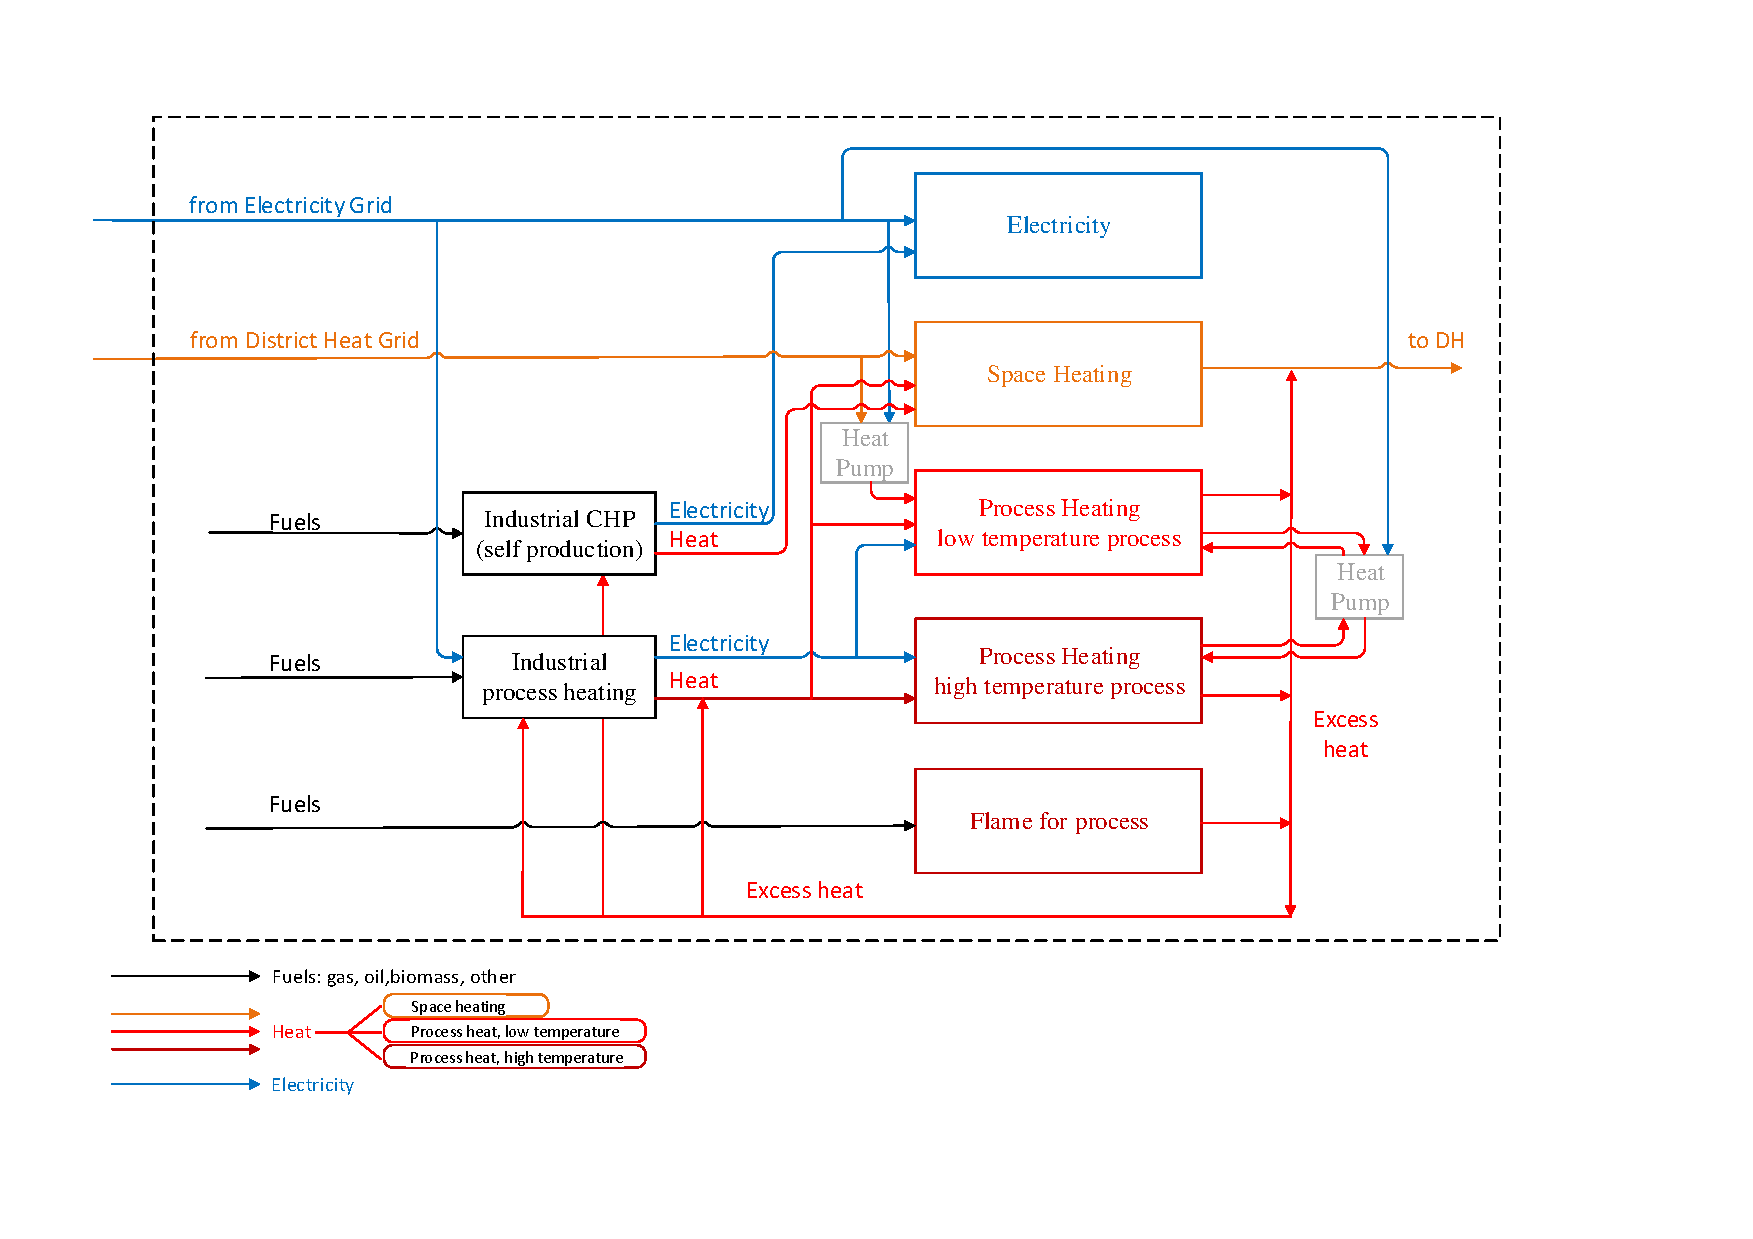
\includegraphics[width=\linewidth]{Img/ind_model/IndustryEnergyFlowchart.pdf}
\caption{Schematic of industry sector representation in Balmorel}
\label{ensyst} 
\end{figure}

The block structure presented in \autoref{ensyst} shows the schematic of the novel structure proposed, to consider the diverse characteristics of the industry sector in the energy system model. The same structure can be applied for each industry group considered. 

The additions introduced concern mainly the commodities part of the energy demand: electricity, fuels and heat.\\
% Electricity 
The electricity supply has to satisfy, in every single sector, the demand of the respective end-uses. This accurate representation facilitates the investigation of end-use specific decarbonisation options (e.g. savings) at a later stage, as the new options can be applied end-use specific. 

Also, electricity can be either be supplied by the grid, or it can be self-produced in on-site industrial plants. It can also be used to run heat pumps and satisfy the heat demand, or "elevate" the quality of heat, for peculiar processes. \\
% Heat
Heat, previously considered only as district heat demand, now includes three temperature levels: space heating, process heat low temperature and process heat high temperature. For this case study, \autoref{tab:temperature_levels} summarises the characteristics of the heat groups, showing how processes are classified according to temperature levels.
Heat can be upgraded (i.e. the temperature is increased) or downgraded (i.e. the temperature is decreased/adapted) using proper heat pumps. 
This means that one can use:
\begin{itemize}
    \item waste heat from a low temperature process to provide heat to a high temperature process
    \item waste heat from high temperature process directly or through a heat pump in a low temperature process
    \item waste heat from a high temperature process to preheat (partly heat) the high temperature process (depending on the temperature considered for low and high temperature processes). 
    \item heat from space heating to provide heat to a low temperature process
\end{itemize}
The excess heat can be used to pre-heat air/water for other processes (e.g. self production) or can be also injected in a DH network where available (i.e. industrial process in proximity to a DH grid). \\
% Fuels
To better represent reality, fuels (used both as energy or fuel-feedstock purposes) are represented directly in the industrial structure with related conversion technologies. This particular facilitates the investigation of CO2 reduction options (like e.g. fuel replacement or electrification) for the industrial sector. \\
%
The modelling of the industry sector requires adaption or extension of different constraints of the energy system model according to the particular considered. The mathematical formulation presented should thus be considered as an extension of the base mathematical model developed for Balmorel (See manual \cite{balmorel}).

\paragraph{Objective function}
The operation of the energy-industry sector implies costs for the energy system. 
As the optimisation in Balmorel is based on cost minimisation (or welfare maximisation if considering elastic demand), the solver minimises the total costs of satisfying the energy demand, while complying with the constraints imposed, based on the best combination of the technologies available. 
The industry-related costs are thus added to the main objective function considering the fuel consumption during the year (\autoref{1}), O\&M of process heat technologies (\autoref{2}), investment in new technologies (\autoref{3}), taxes on investments (\autoref{4}), taxes on emissions (\autoref{5}), taxes on fuel consumption (\autoref{6}), taxes on production of process heat (\autoref{8}) and eventual changes in consumers' utility relative to process heat consumption (\autoref{9}, \autoref{10}). Slack variables are added for detecting infeasibilities (\autoref{11}). 
\begin{align} 
% Cost of fuel consumption during the year
+  & \sum_{a,g,f,s,t,b}C^{fuel}_{af} 3.6 t_{st} q^{ph}_{agstb}  
%& \forall a \in A, \forall g \in G^{ind}, \forall f \in F, \forall s \in S, \forall t \in T 
\label{1}\\ 
%O&M
+  & \sum_{a,g,s,t,b} C^{O\&M}_{ag} t_{st} q^{ph}_{agstb}  
%& \forall a \in A, \forall g \in G^{ind}, \forall f \in F, \forall s \in S, \forall t \in T 
\label{2}\\ 
% Investment costs
+  & \sum_{a,g,c,b} q^{ph-new}_{agb} C^{inv}_{ag} \Lambda_c  
%& \forall a \in A, \forall g \in G^{ind}, \forall c \in C 
\label{3}\\
% Tax on Investment costs
+  & \sum_{a,g,c,b} q^{ph-new}_{agb} C^{tax-inv}_{agb} \Lambda_c 10^6 
%& \forall a \in A, \forall g \in G^{ind}, \forall c \in C 
\label{4}\\
% Tax on Emission
+ & \sum_{a,g,c,s,t,b} t_{st} E^{CO_{2}}_g 10^{-3} 3.6 f^{rate}_{agstb} C^{tax-CO_2}_{c} 
%& \forall a \in A, \forall g \in G^{ind}, \forall c \in C, \forall s \in S, \forall t \in T 
\label{5}\\
% Tax on fuel consumed
+ & \sum_{a,g,c,s,t,f,b} t_{st} C^{tax-fuel}_{fc} 3.6 f^{rate}_{agstb} 
%& \forall a \in A, \forall g \in G^{ind}, \forall c \in C, \forall s \in S, \forall t \in T, \forall f \in F 
\label{6} \\
% Tax on technology type
%+ & \sum_{a}\sum_{g}\sum_{s}\sum_{t} t_{st} c^{tax-gen}_{ag} 3.6 f^{rate}_{agst} & \forall a \in %A, \forall g \in G^{ind},\forall s \in S, \forall t \in T \label{7}\\
% Tax on heat process generation
+ & \sum_{a,g,s,t,b} t_{st} C^{tax-gen-ph}_{ag} 3.6 q^{ph}_{agstb}
%& \forall a \in A, \forall g \in G^{ind},\forall s \in S, \forall t \in T 
\label{8}\\
% Flexibility on heat process demand
+ & \sum_{a,s,t} t_{st} \sum_{down-step} q^{ph-flex}_{ast,ds} C^{down-step}_{ast,ds} 
%& \forall a \in A, \forall g \in G^{ind},\forall s \in S, \forall t \in T,\forall ds \in downstep, 
\label{9}\\
- & \sum_{a,s,t} t_{st} \sum_{up-step} q^{ph-flex}_{ast,us} C^{up-step}_{ast,us} 
%& \forall a \in A, \forall s \in S, \forall t \in T, \forall us \in upstep 
\label{10}\\
%penalties
+ & \sum_{a,s,t} (\Delta^{low}_{ast,low} + \Delta^{up}_{ast,up}) C^{infs} 
%& \forall a \in A, \forall s \in S, \forall t \in T 
\label{11}
%
\end{align}

In Balmorel, the equations are considered for the areas \textit{a}, with the energy producing technologies \textit{g} and fuels \textit{f} available, during the weeks \textit{s} and time steps \textit{t} simulated. The index \textit{b} represents the different temperature levels of process heat, namely space heating (SH), process heat low (PHL) and process heat high temperature (PHH). 
The indexes \textit{us} and \textit{ds} represents the up and down steps in the elasticity demand and the indexes \textit{low} and \textit{up} deals with the upper and lower bounds when considering infeasibility for the equations. 

Variables and parameters are described in \autoref{nomenclature}. 

\begin{table}[H]
\centering
\caption{Nomenclature for the industry modelling}
\label{nomenclature}
\begin{tabular}{lcl}
\hline
Parameters & &  \\ \hline
Name & Unit & Description \\ \hline
$C^{fuel}_{af}$ & \euro /GJ & Fuel price \\
$t_{st}$        & h    & Time steps \\ 
$C^{O\&M}_{ag}$ & \euro/MWh & Operation and maintenance costs \\
$C^{inv}_{ag}$ & \euro/MW & Investment costs \\
$\Lambda_c$ & - & Annuity \\
$C^{tax-inv}_{ag}$ & \euro/MW & Tax on investment costs \\
$E^{CO_{2}}_g$ & kg/GJ & $CO_2$ emission coefficient \\
$C^{tax-CO_2}_{c}$ & \euro/GJ & Tax on $CO_2$ emissions \\
$C^{tax-fuel}_{fc}$ & \euro/GJ & Tax on fuel consumed \\
$C^{tax-gen-ph}_{ag}$ & \euro/GJ & Tax on heat process generation units \\
$C^{up-step}_{ast,us}$ & \euro/MWh & Cost of reduced consumption \\  
$C^{down-step}_{ast,ds}$ & \euro/MWh & Cost of increased consumption \\
$C^{infs}$ & \euro & Infeasibility quota \\
$De^{ind}$ & MWh & Industrial electricity demand \\
$De^{res}_{rst}$ & MWh & Residual electricity demand \\
$De^{ind-elm}_{rstl}$ & MWh & Industrial electricity demand by element \\
$COP_{gb}$ & - & Coefficient of performance \\
$Ph_{astb}$ & MWh & Industrial process heat demand \\
$Q^{ph}_{ag}$ & MW & Capacity installed of process heat technology \\
$F^{eff}_{g}$ & - & Fuel efficiency \\
$F^{MAX}_{cf}$ & GJ & Maximum fuel consumption per country\\
$LIM^{CO_2}_c$ & kg & Maximum $CO_2$ emissions per country \\
\hline
Variables  & &  \\ \hline
$q^{ph}_{agstb}$ & MW & Process heat generation \\
$q^{ph-new}_{agb}$ & MW & New capacity installed \\
$f^{rate}_{agstb}$ & MW & Fuel consumption rate \\
$\Delta^{low}_{ast,low}$ & MW & Slack variable lower bound \\
$\Delta^{up}_{ast,up}$ & MW & Slack variable upper bound \\
$p_{agst}$ & MWh & Electricity generation \\
$q^{DH}_{agst}$ & MWh & District heat generation \\
$q^{ph-flex}_{agstb,ds}$ & MWh & Flexible process heat demand, down steps\\
$q^{ph-flex}_{agstb,us}$ & MWh & Flexible process heat demand, up steps\\

\end{tabular}
\end{table}


\paragraph{Electricity balance}
As illustrated in \autoref{ensyst}, the additional industrial electricity consumption $De^{ind}_{rst}$ related with a region \textit{r} is added to the electricity balance equation in Balmorel according to \autoref{elbalance},

\begin{align}
& \sum_{g} p_{agst} = De^{res}_{rst} + De^{ind}_{rst} \label{elbalance}.
\end{align}

where $De^{res}_{rst}$ is the hourly profile of residual electricity demand not related with industry.

The demand in the industry sector can be satisfied with electricity from the grid or self-production ($p_g, \forall g \in G^{ind}$) and is related with the use of heat pumps and processes/end-uses ($de^{ind-elm}_l, \forall l \in L=\{heat pump, processes\}$):

\begin{align}
& \sum_{l} De^{ind-elm}_{rstl} = De^{ind}_{rst} \label{inddemand}. 
\end{align}

The heat pumps generate heat for the different temperature levels and is related with the electricity use according to \autoref{hprun},

\begin{align}
& De^{ind-elm}_{rst,HP} = q^{ph}_{agstb}/COP_{gb} \label{hprun}.
\end{align}

where $q^{ph}_{agstb}$ is the heat generated from the heat pumps suitable for the temperature levels (SH, PHL, PHH), and $COP_{gb}$ is the coefficient of performance. Heat pumps will have diverse characteristics according to the temperature levels they will work with.


\paragraph{Heat balance}
With the addition proposed, the total heat balance now considers also the heat for industrial purposes provided by the district heating network $Ph_{astb}$ with \textit{b=SH}; the technologies \textit{g} producing heat satisfy the total district heat demand:

\begin{align}
& \sum_{g} q^{DH}_{agst} = Dh^{res}_{ast} + Ph_{astb} \label{dhbalance}
\end{align}

with $Dh^{res}_{ast}$ being the hourly profile of the residual energy system heat demand not related with industry.

Also, industrial DH demand can benefit from heat produced in other processes and self-production.
As presented in \autoref{ensyst}, the heat demand for processes at low and high temperature levels is fullfilled with different set of technologies $g$: district heating grid, self production and other processes for space heating (set $G^{ind-SH}$); heat pumps and industrial processes for low and high temperature process heat (sets $G^{ind-PHH}, G^{ind-PHH}$). Thus a process heat balance is imposed for each of the temperature level proposed:

\begin{align}
& \sum_g q^{ph}_{agstb} = Ph_{astb} & \forall b \in B=\{SH, PHL, PHH\} \label{shbalance}
\end{align}

\paragraph{Process heat related constraints}
\autoref{prcheatbalance} imposes that, at every time step, the production from a set of different technologies meets the heat process demand. Additional variables ($q^{ph-flex}_{agstb,ds}, q^{ph-flex}_{agstb,us}$) allows flexibility in the demand (up and down), while slack variables $\Delta^{low}_{ast,low}, \Delta^{up}_{ast,up}$ are inserted for modelling purposes.


\begin{align}
\sum_{a,g}  q^{ph}_{agstb} = Ph_{astb} &- \sum_{down-step} q^{ph-flex}_{agstb,ds} \notag\\
& + \sum_{up-step} q^{ph-flex}_{agstb,us} - \Delta^{low}_{ast,low} + \Delta^{up}_{ast,up} \label{prcheatbalance}
\end{align}

The fuel consumption rate of the process heat technologies is fixed by \autoref{fuelcons}, where $F^{eff}_{g}$ is the fuel efficiency of technology \textit{g}. 
\autoref{caplimit} imposes limits on the production, i.e. at any time production $q^{ph}_{agstb}$ can exceed capacity $Q^{ph}_{ag}$.

\begin{align}
&  f^{rate}_{agstb} = q^{ph}_{agstb}/F^{eff}_{g} \label{fuelcons} \\
& q^{ph}_{agstb} \leq Q^{ph}_{ag} \label{caplimit}
\end{align}

\autoref{fuelcaplimit} and \autoref{emcaplimit} imposes a cap on fuel consumption and $CO_2$ emissions deriving from the process heat production  per country. $F^{MAX}_{cf}$ represents the maximum fuel use per country. The same constraint in \autoref{emcaplimit} can be used to model emission cap for any other GHG (e.g. $NO_x$ or $SO_2$). The equations can be used used to investigate on the industrial energy mix while complying with future goals on emission reduction and fuel substitution. 

\begin{align}
& \sum_{g,s,t,b} 3.6 t_{st} f^{rate}_{agstb} \leq F^{MAX}_{cf} \label{fuelcaplimit} \\
& \sum_{acgstb} t_{st} E^{CO_{2}}_g 10^{-3} 3.6 f^{rate}_{agstb} \leq LIM^{CO_2}_c \label{emcaplimit}
\end{align}

%%%%%%%%%%%%%%%%%%%%%%%%%%%%%%%%%%%%%%%%%%%%%%
\subsection{Modelling of decarbonisation options}
From a modelling point of view, adding the decarbonisation options in the model influences the optimisation in different ways. 

The electrification of the industry implies a shift from fossil fuels to electricity-based processes. Modelling wise, this means that a new set of process-heat technologies $g$, based solely on electricity $f \in F=\{Electricity\}$, competes with the existing fuel-based technologies. The criteria for the competition can be economic (e.g. the cheapest option for the system, based on \autoref{1}-\autoref{11}), environmental (e.g. cap on $CO_2$ emission, see \autoref{emcaplimit}), or policy based (e.g. imposing share of electrified industrial processes in future energy systems, see \autoref{fuelcaplimit}). Given the constraints imposed, the model then decides the optimal level of investments and operation of the technologies in the energy system.\\ 
The same method applies for the fuel substitution when investigating on the potential use of renewable gasses, biomass and biogas. For this option, the model is given the choice to change the fuel input in existing technologies from the fuels currently in use (e.g. fossil fuels) to more renewable options. Once again, the criteria for selection can be various and includes, among others, availability and proximity to the plant.\\
As a preliminary approach, the wast heat is considered as a free source of heat. Thus, 'blocks' of energy are available for processes at different temperature levels influencing \autoref{prcheatbalance}. Based on the study from \cite{Buhler2017a,Buhler2017}, the excess heat is made available according to the geo-location of the process heat demand (see \autoref{datadescr} for details). \\
Energy savings in the industrial sector act directly on the process heat and industrial electricity demand. Based on the method proposed by \cite{Baldini2016a}, the savings are added as a complementary option. The system has the choice to either supply the energy demand (both electricity and process heat) with the current set of technologies or to invest in energy saving measures, that lower the need for energy. The savings thus impact \autoref{1}-\autoref{11} for the investments costs and \autoref{elbalance}, \autoref{dhbalance}, \autoref{prcheatbalance} for the reduction on electricity, Dh and process heat demand.
The convenience of the investments depends on the value of the savings achieved during the lifetime of the measures versus the cost of supply the energy demand. 


%%%%%%%%%%%%%%%%%%%%%%%%%%%%%%%%%%%%%%%%%%%%%%%%%%%%%%%%%%%%%%%%%%%%%%%%%%%%%%%%%%%%%

\section{Case study / empirical data} \label{datadescr}

%%%%%%%%%%%%%%%%%%%%%%%%%%%%%%%%%%%%%%%%%%%%%%

The possibilities of modelling the industry sector as detailed as described above depend not only on the model structure, but to a great extent on the availability of high resolution data. Data from original sources have to be intensively pre-processed to receive a consistent dataset as model input. Thus in the following the data and its derivation and processing are described.

In this paper, Denmark is taken as a case study for modelling the transition to carbon neutrality in the industrial sector. On the one hand Denmark covers a wide range of different industries but on the other hand the amount of industrial processes still possible to handle to get an impression of the effects of modelling it more in detail in the integrated energy system. Furthermore data availability in Denmark is extensive compared to other countries. This makes it an suitable focus area, in which data processing and modelling methods can be tested with real data, that is still manageable. However, methods can be principally applied to other areas.

\subsection{Overview Data Sources and Processing}
\label{sec:overview_data}
The main input data on Danish industry include fuel demand, end-use specifications, geographical information and potentials of the decarbonisation options. These
\begin{itemize}
 \item Yearly energy demand by industrial group (db117-grouping), fuel type (46 different fuels) \cite{StatisticsDenmark2017}
 \item Energy demand per industry group (57 groups), fuel and end-use for the year 2012 \cite{VM2015} 
 \item Danish companies including address, industry group (db117-grouping) and number of employees \cite{virk2017}
 \item Address database connecting the address to geographic location \cite{aws2017}
 \item Geographic location and extension of district heat areas \cite{kortforsyningen2017}
 \item Hourly gas consumption profiles of gas consumers including the information of the industry group affiliation (db117-grouping) \cite{DanskGasDistribution2016}
 \item Conversion potential of natural gas to electricity and biomass \cite{DGC2013a} and associated costs \cite{DGC2013b}. (Public report: \cite{ENS2014} Appendix 5)
\end{itemize}

As far as possible, openly available data was chosen for the case study. Like that results can be scrutinised based on the open source code and open data. However, consumer profiles can only be published in aggregated form due to confidentiality reasons.

The data flow from original sources to model input is illustrated in \autoref{fig:DataFlow}. The developed scripts are written in python and can be found on Github.
%For the data processing, the python packages pandas and numpy were utilised, which dataframe structure is especially suited for processing and combination of different data source with a satisfactory speed performance. With the objective of achieving a high re-usability and flexibility of data and scripts, the processing was modularised and split in different steps. Between the scripts, intermediate dataframes are passed. This makes the processing more efficient, since some dataframes have to be applied by different subsequent steps. This flow is illustrated in \autoref{fig:DataFlow}.

\begin{figure}[H]
\centering
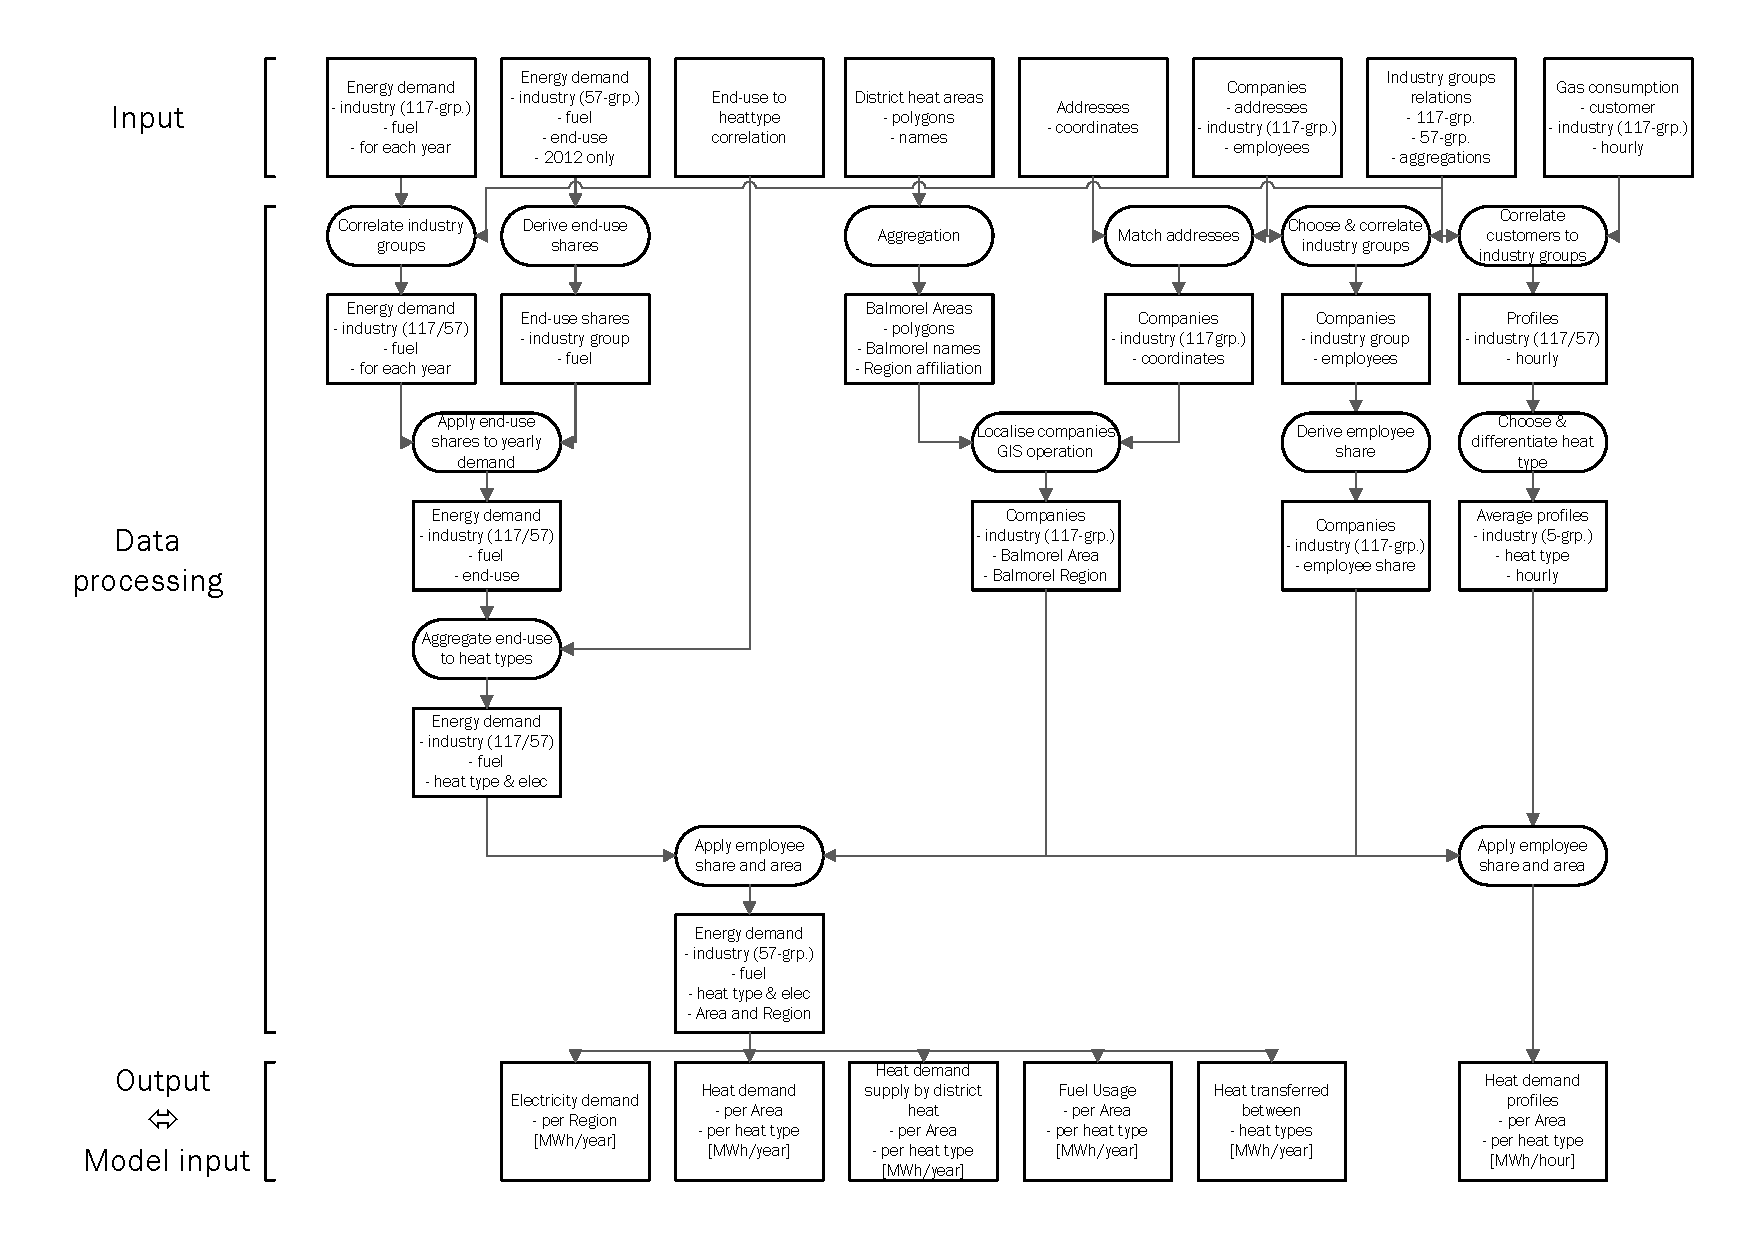
\includegraphics[width=\linewidth]{Img/DataFlow.pdf}
\caption{Data processing from original sources to input for Balmorel. References for the original sources can be found in \ref{sec:overview_data}}
\label{fig:DataFlow} 
\end{figure}

%%%%%%%%%%%%%%%%%%%%%%%%%%%%%%%%%%%%%%%%%%%%%%

\subsection{Energy use by industry groups and fuels}

The Danish national version of EU's nomenclature (NACE) is the Dansk Branchekode DB07 (Danish Branch Code), a statistical classification of economic activities that categorises each enterprise based on its main activity \cite{DanmarksStatistik2013}. The energy consumption by industry group and fuel type is published by Statistics Denmark on a yearly basis \cite{StatisticsDenmark2017}. This data is reliably and continuously available and the structure of the industry grouping follows the db117-code which is widely applied in Denmark for identifying the affiliation of companies and utilised in other data sources about the conversion potential in industry.

As described and shown above (\autoref{sec:energy_use}), detailed figures on end-use are available from a \cite{VM2015} for 57 sectors, 22 end-use processes and 20 type of fuels but just for the year 2012 .

Thus, the shares each end-use consumes per fuel and industry group, derived from \cite{VM2015} were applied to the absolute numbers on fuel use per industry group from Statistics Denmark. Due to the fact, that the industry groups were chosen slightly different than in Statistics Denmark, these had to be correlated. Additionally, fuel naming had to be aligned and partly aggregated. The calculation flow is illustrated in \autoref{fig:DataFlow}.

The resulting numbers for 2014 and 2015 show that energy use in agriculture did not change significantly ($\sim$19 PJ), while service after a decrease in 2014 ($\sim$46 PJ) increased to an almost similar level like 2012 in 2015 ($\sim$48 PJ). Energy use in production single shift stays on the same level ($\sim$5 PJ), production double shift decreased from 2012 ($\sim$44 PJ) to 2014 ($\sim$41 PJ), rising again in 2015 ($\sim$43 PJ) and production triple shift decreased to ($\sim$38 PJ). In total, energy use for heat and electricity (excluding transport) sum up to $\sim$148 PJ in 2014 and $\sim$152 PJ in 2015.

With regard to fuels, a slight increase in electricity use can be noted from $\sim$59 PJ in 2012 to $\sim$61 PJ in 2015. In the same time-span, use of natural gas decreased from $\sim$35 PJ to $\sim$32 PJ and delivered heat from $\sim$26 PJ to $\sim$23 PJ. This could be a sign for a slight increase in electrification of heat in industry.

%For the groups of economic activities, detailed data on yearly energy usage by fuel type is available. A detailed clustering on the end-use of the fuels utilised is provided in \cite{VM2015}, but just for 57 groups excluding public service, mining and construction. The allocation of economic activities to the sectors mainly follows the grouping from Statistics Denmark; the exact allocation can be found in the Annex of \cite{VM2015}. 
%\\
%The consumption of the 57 sector is available as a total of 22 end-use processes supplied by 20 types of fuels.  \cite{VM2015}.
%\\

% This calculation can be applied to each available year of the Statistics Denmark data, so that after this calculation step, the energy usage per industry group, fuel and end-use is available for different years. It has to be mentioned that the division has to be adapted if the end-use within an industry group changes significantly. Growth of industry groups and thus energy usage increase would be divided by the same end-use allocation.

%From that dataset, public service, building and mining was excluded.

%On the end-use side, transport of all industry groups is excluded from the dataset and the case study focuses on electricity and heat demand.

%The required temperature level is decisive for which conversion options are available to reduce the use of fossil fuels. The allocation of the fuel usage in industry to different end-use categories is available for the year 2012 from the ... for a large part of Danish industry. The absolute fuel consumption numbers per end-use, fuel and industry group were converted to shares relating to industry groups and fuel usage. Due to the fact that the industry groups were chosen slightly different than in Statistics Denmark, this had to be accounted for. Also, fuels and industry grouping had to be aligned. 

\subsection{Heat levels}
Derived from the conceptual model, we group the end-use heat demand into space heat, process heat low and process heat high. This was considered detailed enough to capture the main differences between the conversion option while still model-wise manageable. Nine end-use heat categories were available from the main data, which are - depending on their required temperature level aggregated as displayed in Table \autoref{tab:temperature_levels}.

\begin{table}
\begin{tabular}{l | c | c}
End-use & Temperature level [$^{\circ}$C] & Model heat type\\
\hline \hline
Space heating & 50-90 & space  \\ 
Distillation & 50-100 & process low \\
Heating/Boiling & mostly 70-110 & process low \\
Drying & about 100 & process low \\
Inspissation & 130 & process low \\ 
Burning/Sintering & more than 250 & process high \\ 
Melting/Casting & more than 300 & process high  
\end{tabular}
\caption{Clustering end-use by heat level. Source for process heat levels: \cite{VM2015}}
\label{tab:temperature_levels} 
\end{table}

In 2015 space heat accounts for $\sim$34 PJ in industry, process heat low temperature for $\sim$44 PJ and process heat high temperature for $\sim$13 PJ.

%%%%%%%%%%%%%%%%%%%%%%%%%%%%%%%%%%%%%%%%%%%%%%

\subsection{Profiles}
\label{sec:profiles}

The temporal patterns of electricity and heat demand need to be adequately represented by the input data for industry modelling. Realistic profiles are necessary to capture the effects of varying electricity prices due to increasing shares of fluctuating electricity sources like wind and solar energy.

The five aggregated industry groups agriculture, service, production singe, double, triple shift follow different temporal patterns as described in \autoref{inddescr}. This categorisation, as well as underlying assumptions, are based on \cite{VM2016} and especially convenient to distinguish profiles for the demand of these groups. 

Electricity, space and process heat profiles differ significantly. While demand for process heat is process dependent, space heat follows a strong seasonal pattern. Thus, for each of these, profiles for each of the five groups are required.

The profiles required for model input are derived from real data for electricity, space heat and process heat for the detailed industry groups. Subsequently these are aggregated to the five groups. The methods and a thorough description of the data sources can be found in\cite{Wiese2017} and the resulting profiles are described in the following.

\subsubsection{Demand profiles: Electricity}

The following figures show an evaluation of the resulting electricity profiles for the five groups. The temporal variation differs significantly. On the y-axis, the share of electricity consumption in each hour of the yearly consumption is given. Thus, the boxplots (\autoref{boxplots}) illustrate the temporal variability. As expected, the temporal variability is highest for agriculture and lowest for the production working in triple shift. Looking at the yearly variation (\autoref{trendlines}), agriculture shows a high variation.

\begin{figure}[H]
\centering
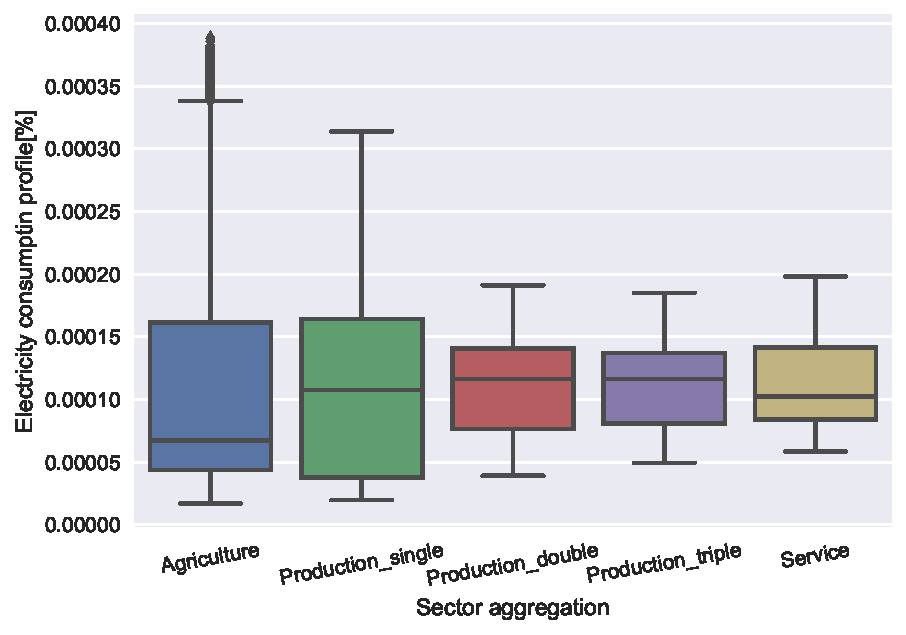
\includegraphics[width=\linewidth]{Img/profiles/boxplots.pdf}
\caption{Boxplots of relative electricity consumption. Own calculations based on \cite{Energinet.dk,NordPool2016,ElforbrugsPanelerne2015,Andersen2013a,Andersen2013b,VM2015}}
\label{boxplots} 
\end{figure}

\begin{figure}[H]
\centering
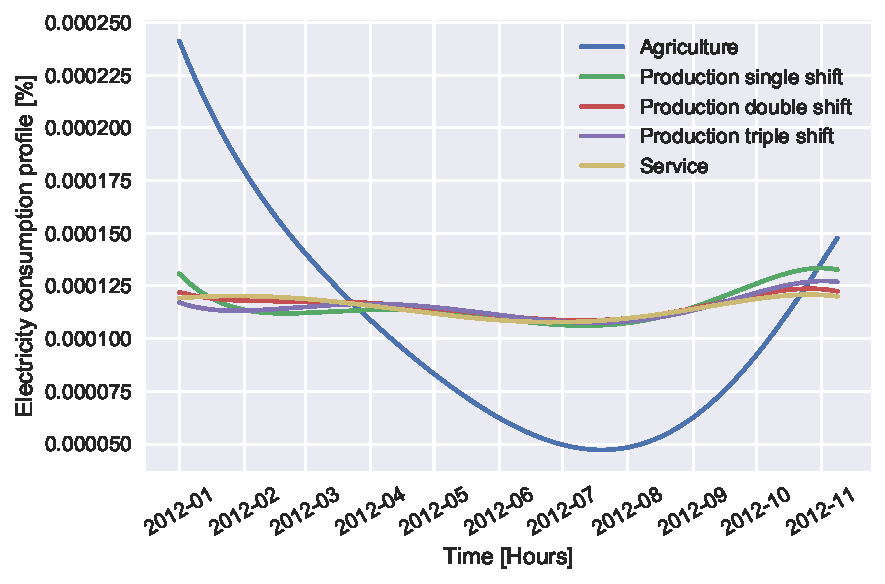
\includegraphics[width=\linewidth]{Img/profiles/trendlines.pdf}
\caption{Relative variation of seasonal electricity consumption, trend-lines (fit to the 18th order). Own calculations based on \cite{Energinet.dk,NordPool2016,ElforbrugsPanelerne2015,Andersen2013a,Andersen2013b,VM2015}}
\label{trendlines}
\end{figure}

\subsubsection{Demand profiles: Space Heat}

For space heat, there is a clear indication of the seasonal and the weekly variation. The expected seasonal variation can be seen in \autoref{heat_space_year}. On a weekly basis (\autoref{heat_space_week}), the triple shift production sector shows the smallest variation.

\begin{figure}[H]
\centering
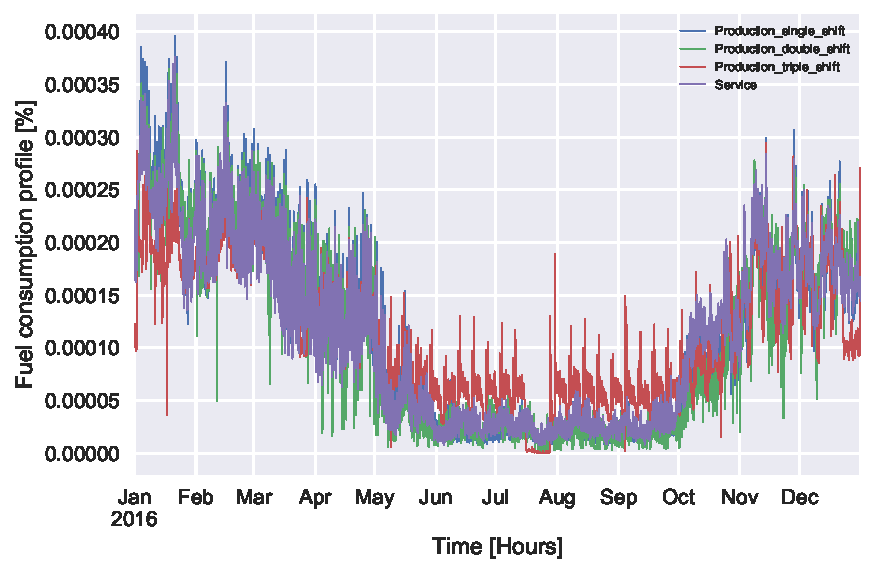
\includegraphics[width=\linewidth]{Img/profiles/heatprofile_space_year_perc.pdf}
\caption{Yearly scale. Own calculations based on data from \cite{DanskGasDistribution2016,VM2015}}
\label{heat_space_year}
\end{figure}
	
\begin{figure}[H]
\centering
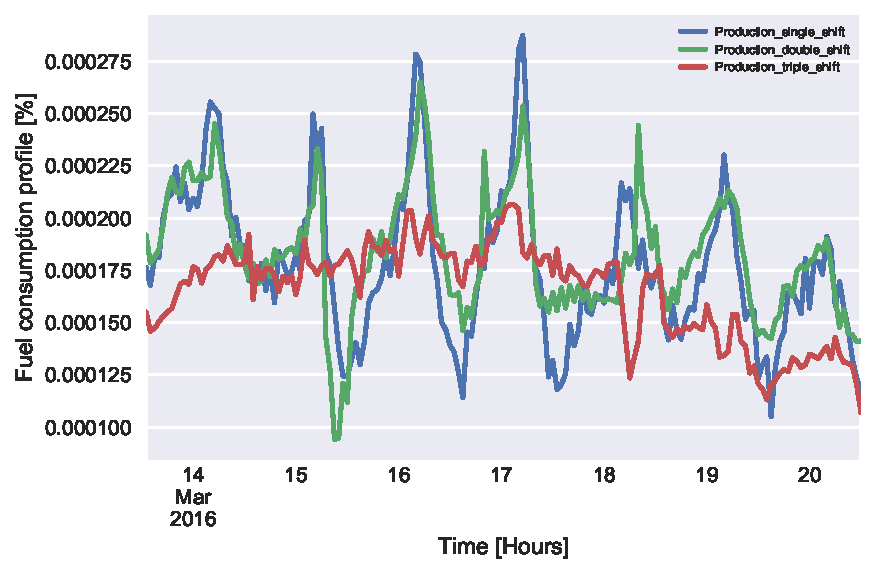
\includegraphics[width=\linewidth]{Img/profiles/heatprofile_space_week_perc_noserv.pdf}
\caption{Sample week. Own calculations based on data from \cite{DanskGasDistribution2016,VM2015}}
\label{heat_space_week}
\end{figure}

\subsubsection{Demand profiles: Process heat}
For process heat, the yearly picture (\autoref{heat_process_year}) supports the approach of utilising real data instead of constructed profiles, since these specific shape demonstrates that holidays have a huge impact on the demand: During Easter, Summer and Christmas holidays, the demand is significantly lower. For energy system analysis all these special situations are especially interesting since they could cause special situation of oversupply, negative prices, etc. \autoref{heat_process_week} illustrates the different weekly routine of triple, double and single shift production and the subsequent differences in energy demand profiles. 

\begin{figure}[H]
\centering
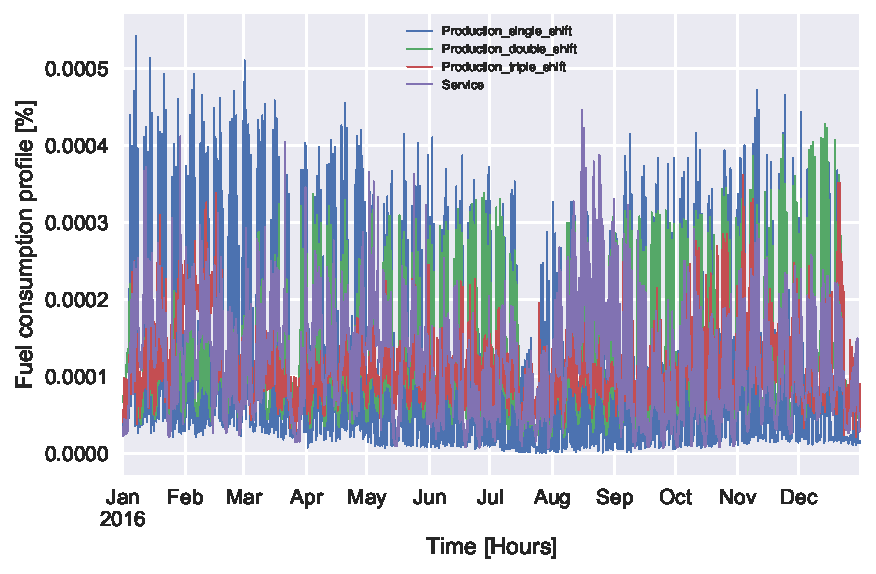
\includegraphics[width=\linewidth]{Img/profiles/heatprofile_process_year_perc.pdf}\\
\caption{Yearly scale. Own calculations based on data from \cite{DanskGasDistribution2016,VM2015}}
\label{heat_process_year}
\end{figure}
	
\begin{figure}[H]
\centering
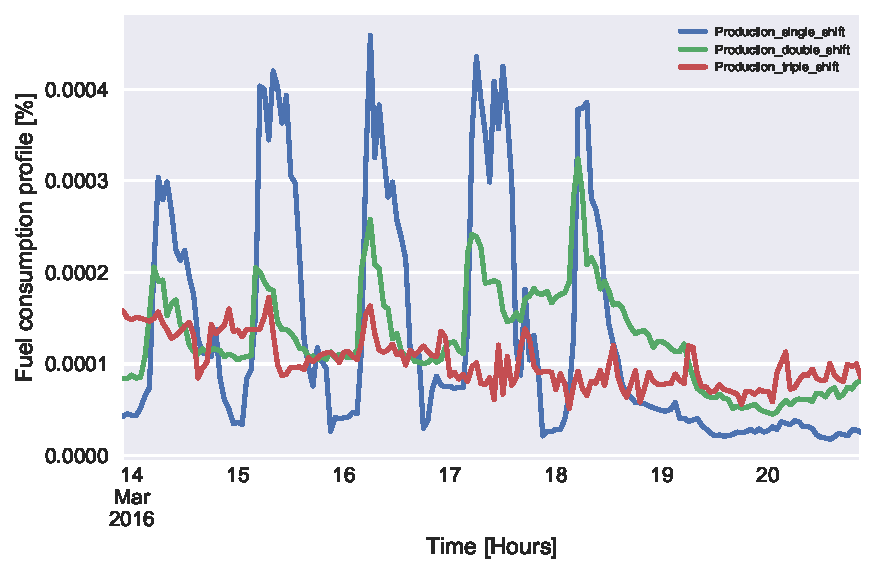
\includegraphics[width=\linewidth]{Img/profiles/heatprofile_process_week_perc_noserv.pdf}\\
\caption{Sample week. Own calculations based on data from \cite{DanskGasDistribution2016,VM2015}}
\label{heat_process_week}
\end{figure}

%%%%%%%%%%%%%%%%%%%%%%%%%%%%%%%%%%%%%%%%%%%%%%

\subsection{Geographical mapping of industrial energy consumption}

District heating plays a major role in Denmark. Approximately 60\% of the Danish heating needs is supplied via district heat networks while 40\% of fuel consumption is based on renewable sources \cite{Munster2012}. In line with the Danish goal to be independent of fossil fuels in 2050, the supply of district will be transformed to completely renewable sources. Generally district heating infrastructure facilitates an efficient fuel use. Supposing a further increasing share of renewable sources in district heating, an increased use of district heat for and process heat for industry is an important option to reduce fossil fuel usage. The feasibility of this option depends on the location of this industrial demand. Whether the company is located within or in vicinity to a district heating area decides whether this option can be used. Depending on the required temperature, heat pumps would be necessary to raise the provided temperature. The vicinity to such a network is furthermore decisive for the possibility of excess heat usage. Connection to a district heat network offers the possibility to exploit the otherwise lost heat potential beyond recycling it on site.

It is not only necessary to determine which part of industrial energy demand and excess heat can be connected to district heat in general, but also to which district heat area. Following the logic of the model Balmorel, heat can just be distributed within an Area in Balmorel. If the geographical relation between heat source and heat demand would disregarded, the effort of matching heat demand and supply temporarily would be underestimated and the potentials for district heat and usage of excess heat overestimated. The modelled 36 Balmorel Areas in this study are aggregated real Danish district heat areas. Connected district heat areas are aggregated and small rural district heat areas are summarised for Denmark East and Denmark West. This aggregation is a compromise between model complexity / calculation time and accuracy. Since mostly small areas are summarised, the effect on the results is minor.

Concluding, the location of industrial heat utilisation related to district heat areas is thus crucial as input data for the Danish case.

The basis of this localisation is the list of companies located in Denmark which includes addresses, affiliation to detailed industry group and number of employees information \cite{virk2017}. Entries that did not have any employees reduced the number of companies from 817.064 to 390.426. The geographic location (coordinates) for the remaining were derived by matching the addresses to an address list containing coordinates \cite{aws2017}. This was done via a matching operation in python. District heat areas in Denmark are provided publicly as a shape-file \cite{forsyningsomraade2017} and were aggregated to the 36 areas as described in \cite{Petrovic2014}. Via the coordinate information, the companies were assigned an area with a spatial join operation in the geographical software QGIS.

The method for localisation of the industrial energy demand by fuel and end-use is based on the employee shares of industrial groups of companies. This method has first been used by \cite{Buhler2017} including a verification description of the method. The number of employees is not proportional to the energy used if considering companies of different industry groups, e.g. a company of a work intensive group like service will have more employees per MWh/year than a production facility with high automation. However, the more detailed the distinction between industry groups is, the more similar is the employee/energy ratio of the companies withing the respective industry group. The described grouping into 57 industry groups is considered sufficient detailed for assuming that the number of employees is proportional to the energy usage within the respective industry group.

As indicated in the data flowchart (\autoref{fig:DataFlow}), the share of employees in relation of the sum of employees in the respective industry group was calculated for each company. Subsequently, the yearly energy demand per fuel and end-use for each industry group was assigned to the companies via the employee share. The area in which a company is located is defined by the preceding calculation. Thus, the energy demand per fuel and end-use can be summed for each model area. This is a direct input for the model.

%iffalse
% \begin{figure}[H]
% \centering
% 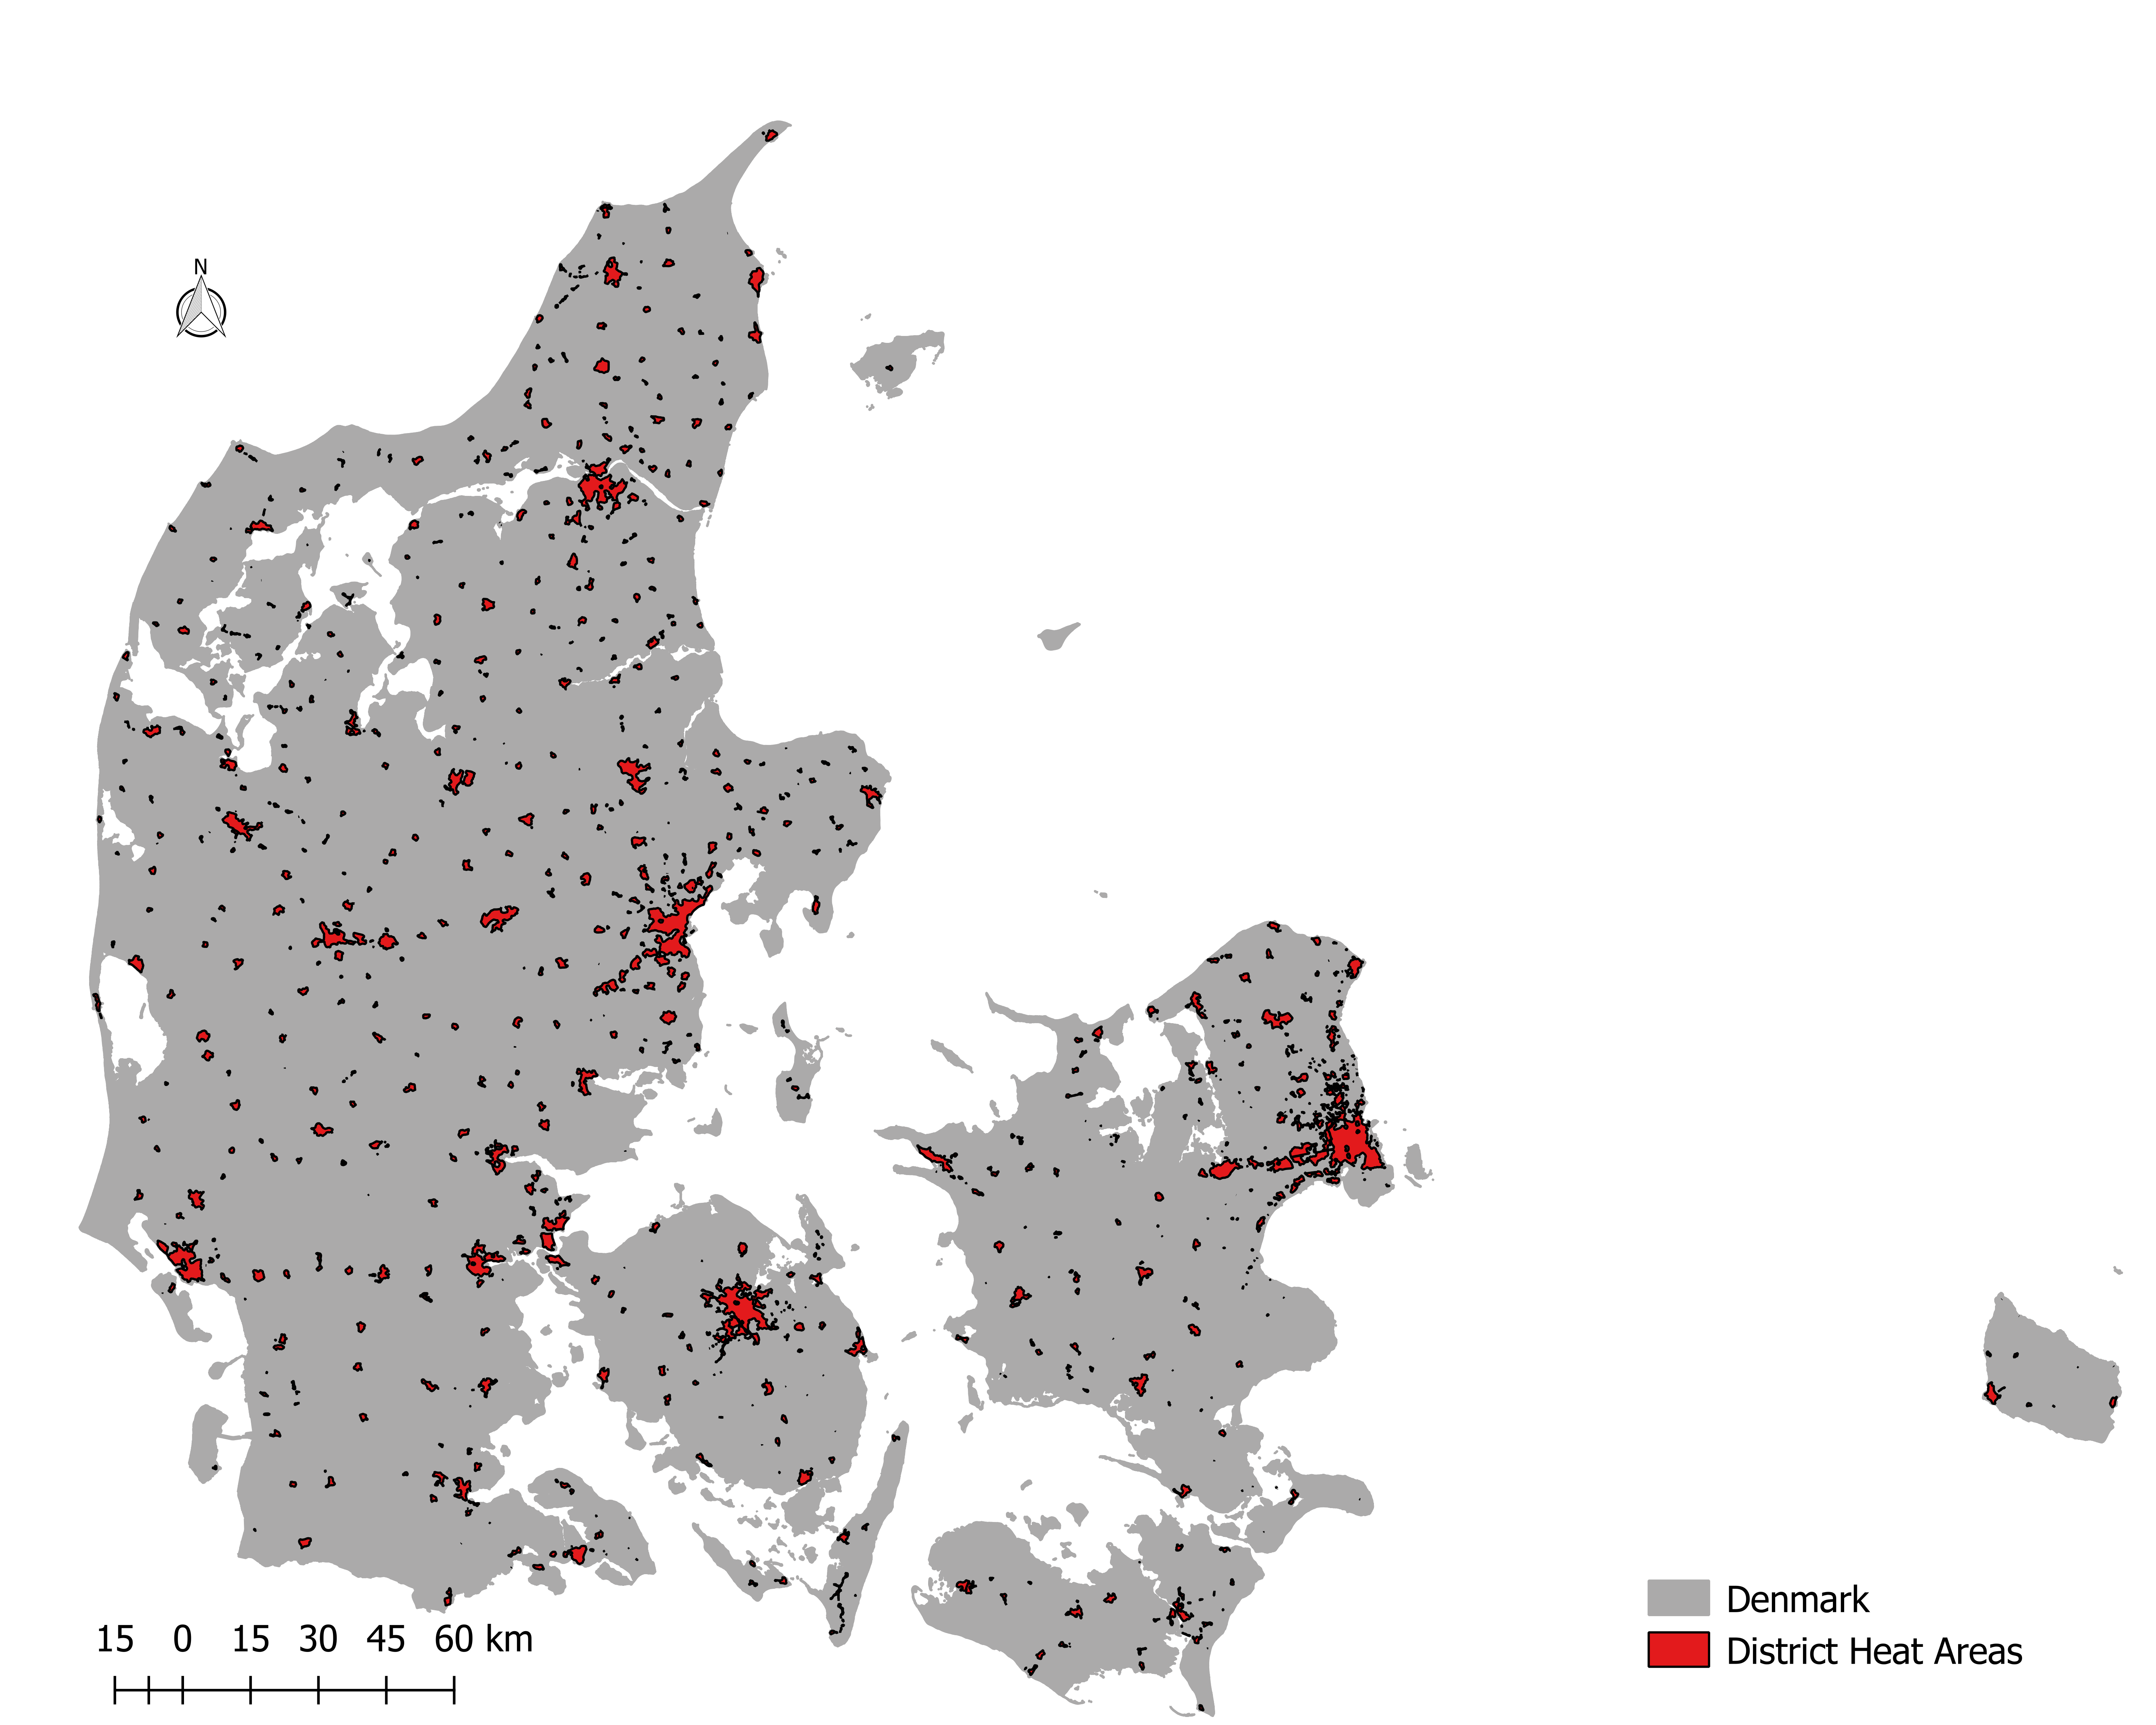
\includegraphics[width=\linewidth]{Img/geo/DK_DH_Balmorel_areas2.png}
% \caption{District Heat Areas in Denmark. Sources: \cite{kortforsyningen2017,forsyningsomraade2017}}
% \label{fig:DH}
% \end{figure}

% \begin{figure}[H]
% \centering
% \includegraphics[width=\linewidth]{Img/geo/DK_DH_Balmorel_areas2_companies.png}
% \caption{Location of Companies. Own processing based on: \cite{kortforsyningen2017,virk2017,aws2017,Buhler2017}}
% \label{fig:DH_Balmorel}
% \end{figure}

%The official Danish district heat areas (Figure \ref{fig:DH}) are for model complexity reduction aggregated in a way that district heat areas that in reality have a connections are summarised and all small rural areas are modelled as one. Figure \ref{fig:DH_Balmorel} shows all companies in Denmark that were located to the modelled district heat areas. 

The resulting space heat demand within district heat areas sums up to $\sim$17 PJ of which $\sim$11 PJ are already supplied by district heat. The remaining $\sim$16 PJ space heat demand is located outside current district heat areas. \autoref{fig:DH_SH_share}) illustrates the share of space heat demand that is supplied by district heat for the modelled 36 areas. The share per area ranges from 40-80\%. For a clearer illustration, the summarised rural district heat areas with minor heat demand are excluded in the figure.

About 10 PJ process heat demand of low temperature is located within district heat areas and  $\sim$33 PJ outside. For process heat lower temperature the share already supplied by district heat ranges between 0 and 30\% for the different areas as shown in \autoref{fig:DH_PHL_share}.

For process heat of high temperature, the localisation within a district heat network increases the possibility to use excess heat by injecting it into the district heat network. About 3 PJ are located within while $\sim$10 PJ are located outside current district heat areas.

These numbers indicate an upper limit for connection to district heat on the supply but also on the excess heat side. It has to be mentioned that so far, that so far just localisation within a district heat area is considered. A possible extension of the district heat grid could extent the potential and thus

\begin{figure}[H]
\centering
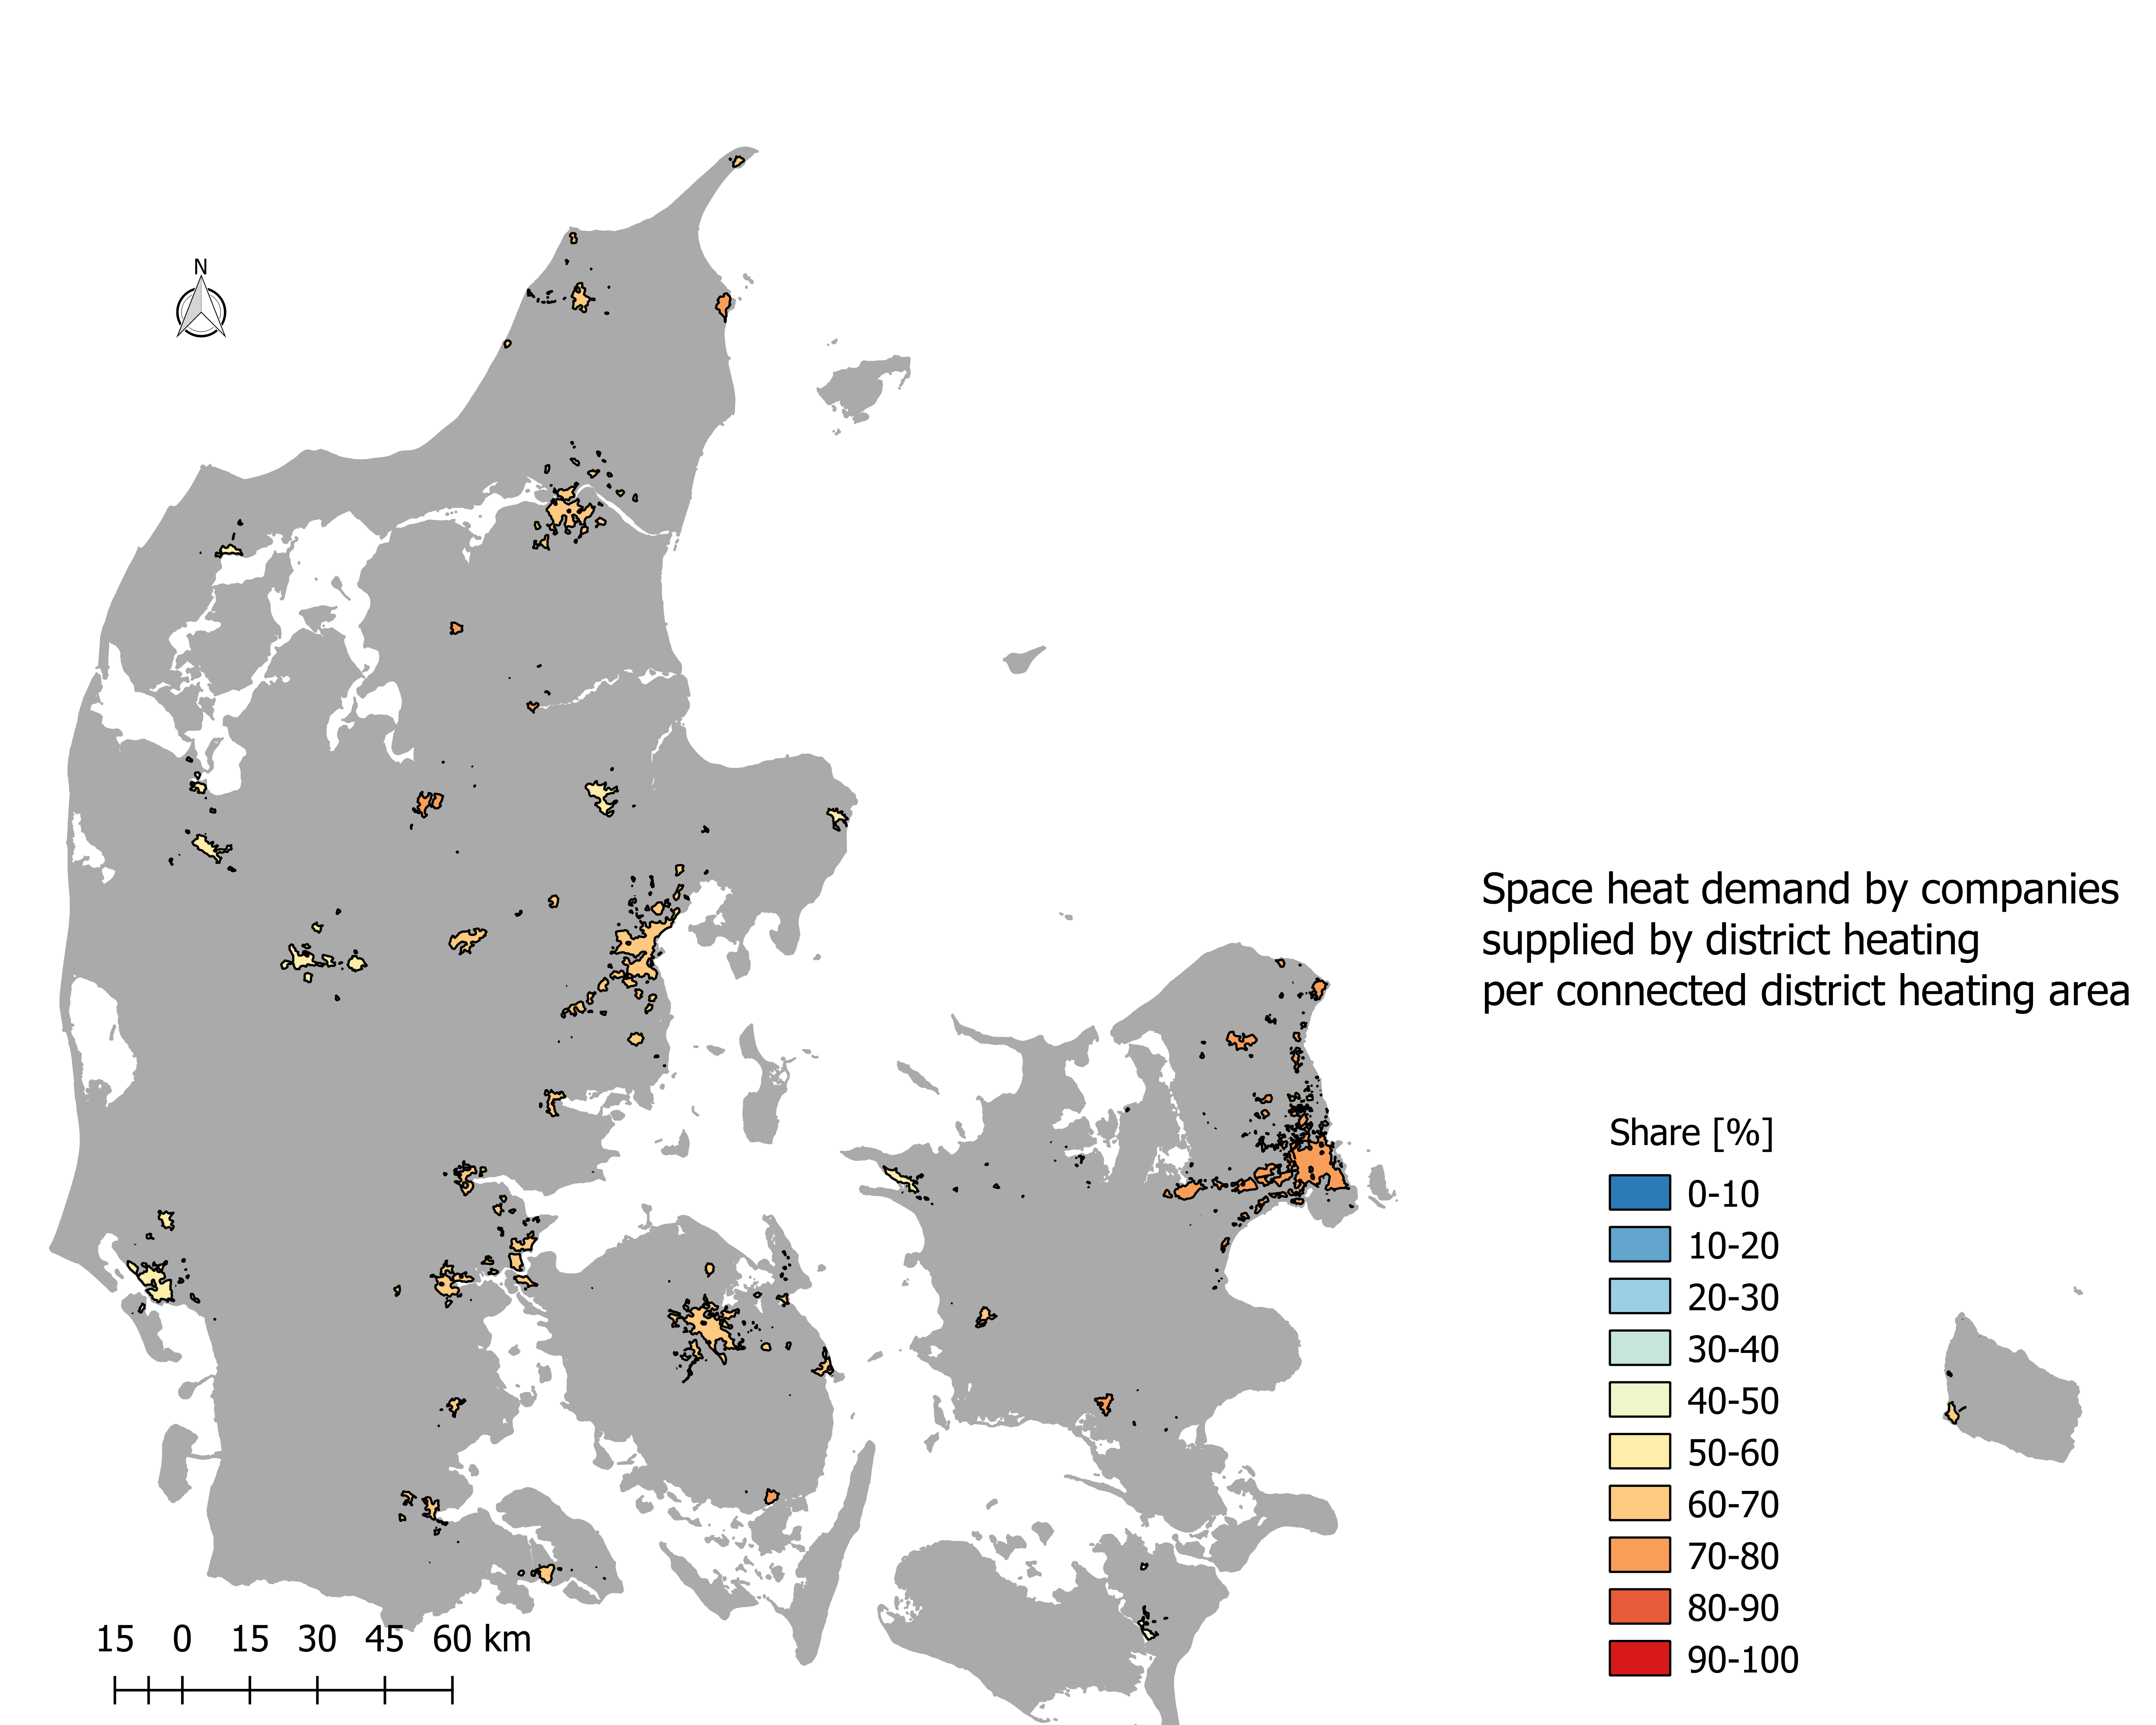
\includegraphics[width=\linewidth]{Img/geo/DK_DH_Balmorel_areas2_DH_share_SH.png}
\caption{Space heat demand of companies supplied by district heat. Own calculations based on: \cite{kortforsyningen2017,virk2017,Buhler2017,Petrovic2014,VM2015,StatisticsDenmark2017}}
\label{fig:DH_SH_share}
\end{figure}

\begin{figure}[H]
\centering
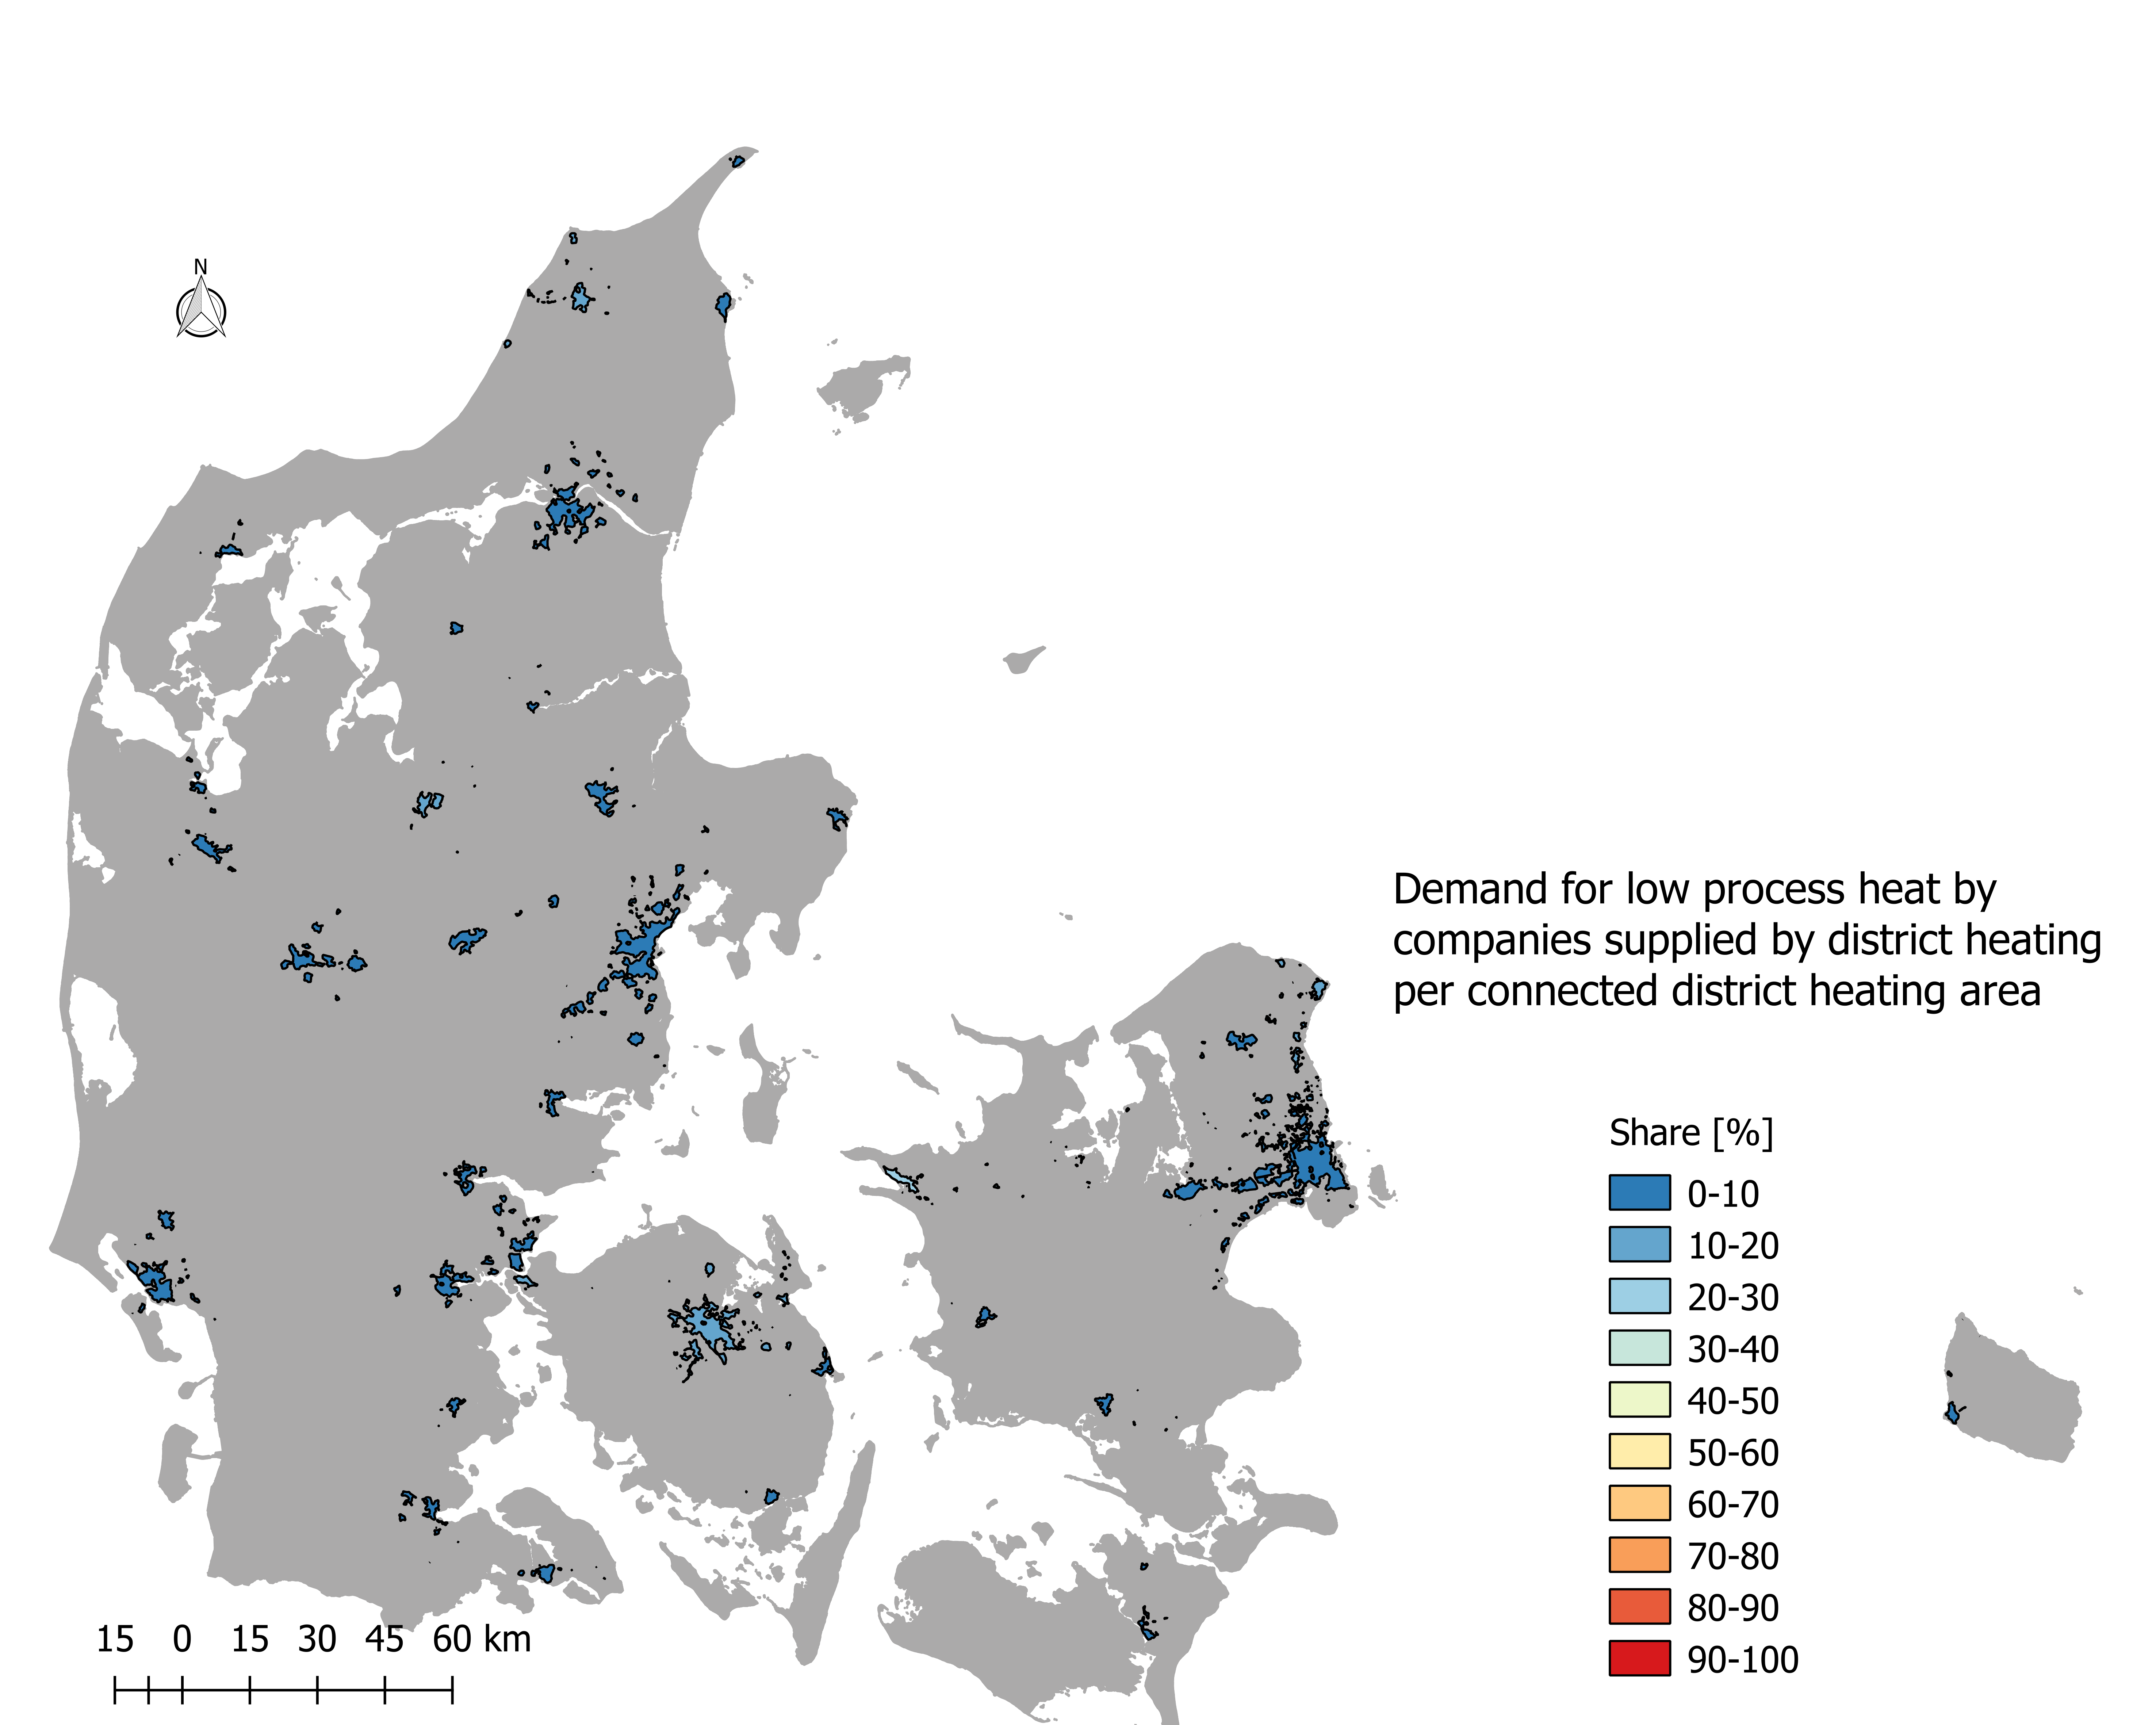
\includegraphics[width=\linewidth]{Img/geo/DK_DH_Balmorel_areas2_DH_share_PHL.png}\\
\caption{Low process heat demand supplied by district heat. Own calculations based on: \cite{kortforsyningen2017,virk2017,Buhler2017,Petrovic2014,VM2015,StatisticsDenmark2017}}
\label{fig:DH_PHL_share}
\end{figure}
%fi

A similar approach is applied to derive the demand profiles per area. For each area, the profiles described in \autoref{sec:profiles} are applied proportionally to the electricity, space and process heat demand of the five main industry groups.

Electricity demand and its temporal profile just have to be defined on a regional level, which include several areas in the model logic. Within Balmorel Regions, transmission of electricity cannot be restricted. Since this is just possible for electricity flow between regions, these should be chosen in a way that potential bottlenecks are represented between regions. Following that rule, Denmark is modelled in two regions: Denmark East including Zealand and Denmark West including Jutland and Funen. Thus the same approach as described for heat in areas in applied in regions for localisation of electricity demand data.

%%%%%%%%%%%%%%%%%%%%%%%%%%%%%%%%%%%%%%%%%%%%%%

\subsection{Decarbonisation option potentials}

\textit{maybe a table with the different options and if they are applicable for process heat high, low and space heat and make an indication if they are rather expensive or rather cheap / subsection could also be before geographical subsection}
% Biomass: get price range and maybe the potential for DK?
% Biomass: see VE til process for biomass cost assumption
\begin{table}
\small{
\begin{tabular}{l | c | c | c | c}
Decarbonisation & Space heat & Process heat & Process heat & Electricity \\
category & & low & high & \\
\hline \hline
Energy savings & \textit{rough potential} & \textit{rough potential} & \textit{rough potential} & \textit{rough potential}\\

Excess heat & na & if in DH-area & if in DH-area & na\\
usage &&&&\\
%District heat & if in DH-area & if in DH-area; & na & na \\
%&& heat pump required &&\\
Electrification & Heat pump & Heat pump or & Electric heat & na\\
&& electric heat &&\\
Biomass & price range: & price range: & same as for PHL & main energy\\
& restricted potential: & restricted potential: && system\\
Biogas & if close to source & dep. on devices/ & dep. on devices/ & main energy\\
&& gas quality & gas quality & system\\
Renewable gas &  12 Euro/GJ  & 12 Euro/GJ & 12 Euro/GJ & decided on\\
& \cite{EA2017,Jensen2017b,Bramstoft2017} &&& system level\\
\end{tabular}
\caption{Overview of decarbonisation options in industrial energy use}
\label{temperature_level} 
}
\end{table}

Heat pumps play decisive roles as the overview table show. It has to be noted that it is decisive for the modelling to distinguish the technical properties and the coefficient of performance (COP) according on the application area. Heat pumps are available for different temperature levels and their COP differs depending on input and output temperature. From \cite{VM2015}, COP of heat pumps can be roughly derived per industry group by dividing the heat output by the electricity output. These numbers can be utilised as check values for the heat pump assumptions.

As long as the industry receives electricity from the main grid, it depends on the electricity supply system how high the renewable share is in the electricity mix and how expensive the electricity is. In the model maximising social welfare, saving options can thus directly compete cost-wise. This stresses the importance of modelling industry within the integrated energy system and not isolated.

For electrification options, \textit{cite DGC-report} was taken as input. This study defines the electrification potential in shares for different technology types. It is based on a database including all gas appliances in Denmark with their installed capacity and amount of gas consumed yearly. In the background report, it is described which industry groups use which technology. The electrification potential is defined by the cubic-meter gas per year consumed. Processes that need a flame cannot be electrified. These are in Denmark for example \textit{Translate: This is Krympeplast, flammehærdning, glasfiberproduktion, skæring}. However, the percentage is rather low and just sums up to about 1~\% of gas usage in Denmark. Processes with high temperature are typically in \textit{Translate:teglværker, cementovne, glasindustrien samt ved produktion af isoleringsmaterialer I virksomheder med støbe- og smelteprocesser ses højtemperaturbrændere også} If high temperatures are transferred to heat by radiation and the \textit{translate: røggasserne ikke kommer i direkte kontakt med materialet i processen}, it is possible to replace the flame by electricity. However, \textit{translate: Ovne, der bruger røggasbortledningen som en del af varmefordelingen, fx forvarmning, kan også være problematiske}.
Generally processes with require radiaton are straightforward to electrify. A large share of gas is utilized for hot water and damp for processes. These are for example required in \textit{Translate: Slagterier, fremstilling af olier og fedtstoffer, fremstilling af mejeriprodukter, fremstilling af færdige foderblandinger, fremstilling af fortykningsmidler (pektin) m.v.}. A direct change to electricity is not as straightforward as for radiation. A more detailed analysis of the circumstances and the temperatures would be required.
In total, according to \cite{DGC2013a} 78-85~\% of the gas utilised in industry could be converted. There is some uncertainty especially about the hot water and damp generation, but for the preliminary analysis, it is assumed .......?

The costs for switching to electricity is estimated in \cite{DGC2013b}, summarised for the same technology groups. The installation costs do not only include the appliance costs, but also the electricity grid connection or enforcement costs respectively. Matched to the industry grouping utilised in our analysis, this cost assumptions are utilised as input for the model.

%%%%%%%%%%%%%%%%%%%%%%%%%%%%%%%%%%%%%%%%%%%%%%%%%%%%%%%%%%%%%%%%%%%%%%%%%%%%%%%%%%%%%

\section{Preliminary results} \label{outcdisc}

\begin{table}[H]
\centering
\caption{Investigation of decarbonisation options in industry sector}
\label{results}
\begin{tabular}{llll}
\hline
 & Electrification & Savings & Fuel replacement \\
\hline
$CO_2$ emissions [\%] &  &  &   \\
Electricity consumption [\%] &  &  &   \\
System costs [\%] &  &  &   \\
\hline
\end{tabular}
\end{table}

\iffalse
\begin{figure}[H]
\centering
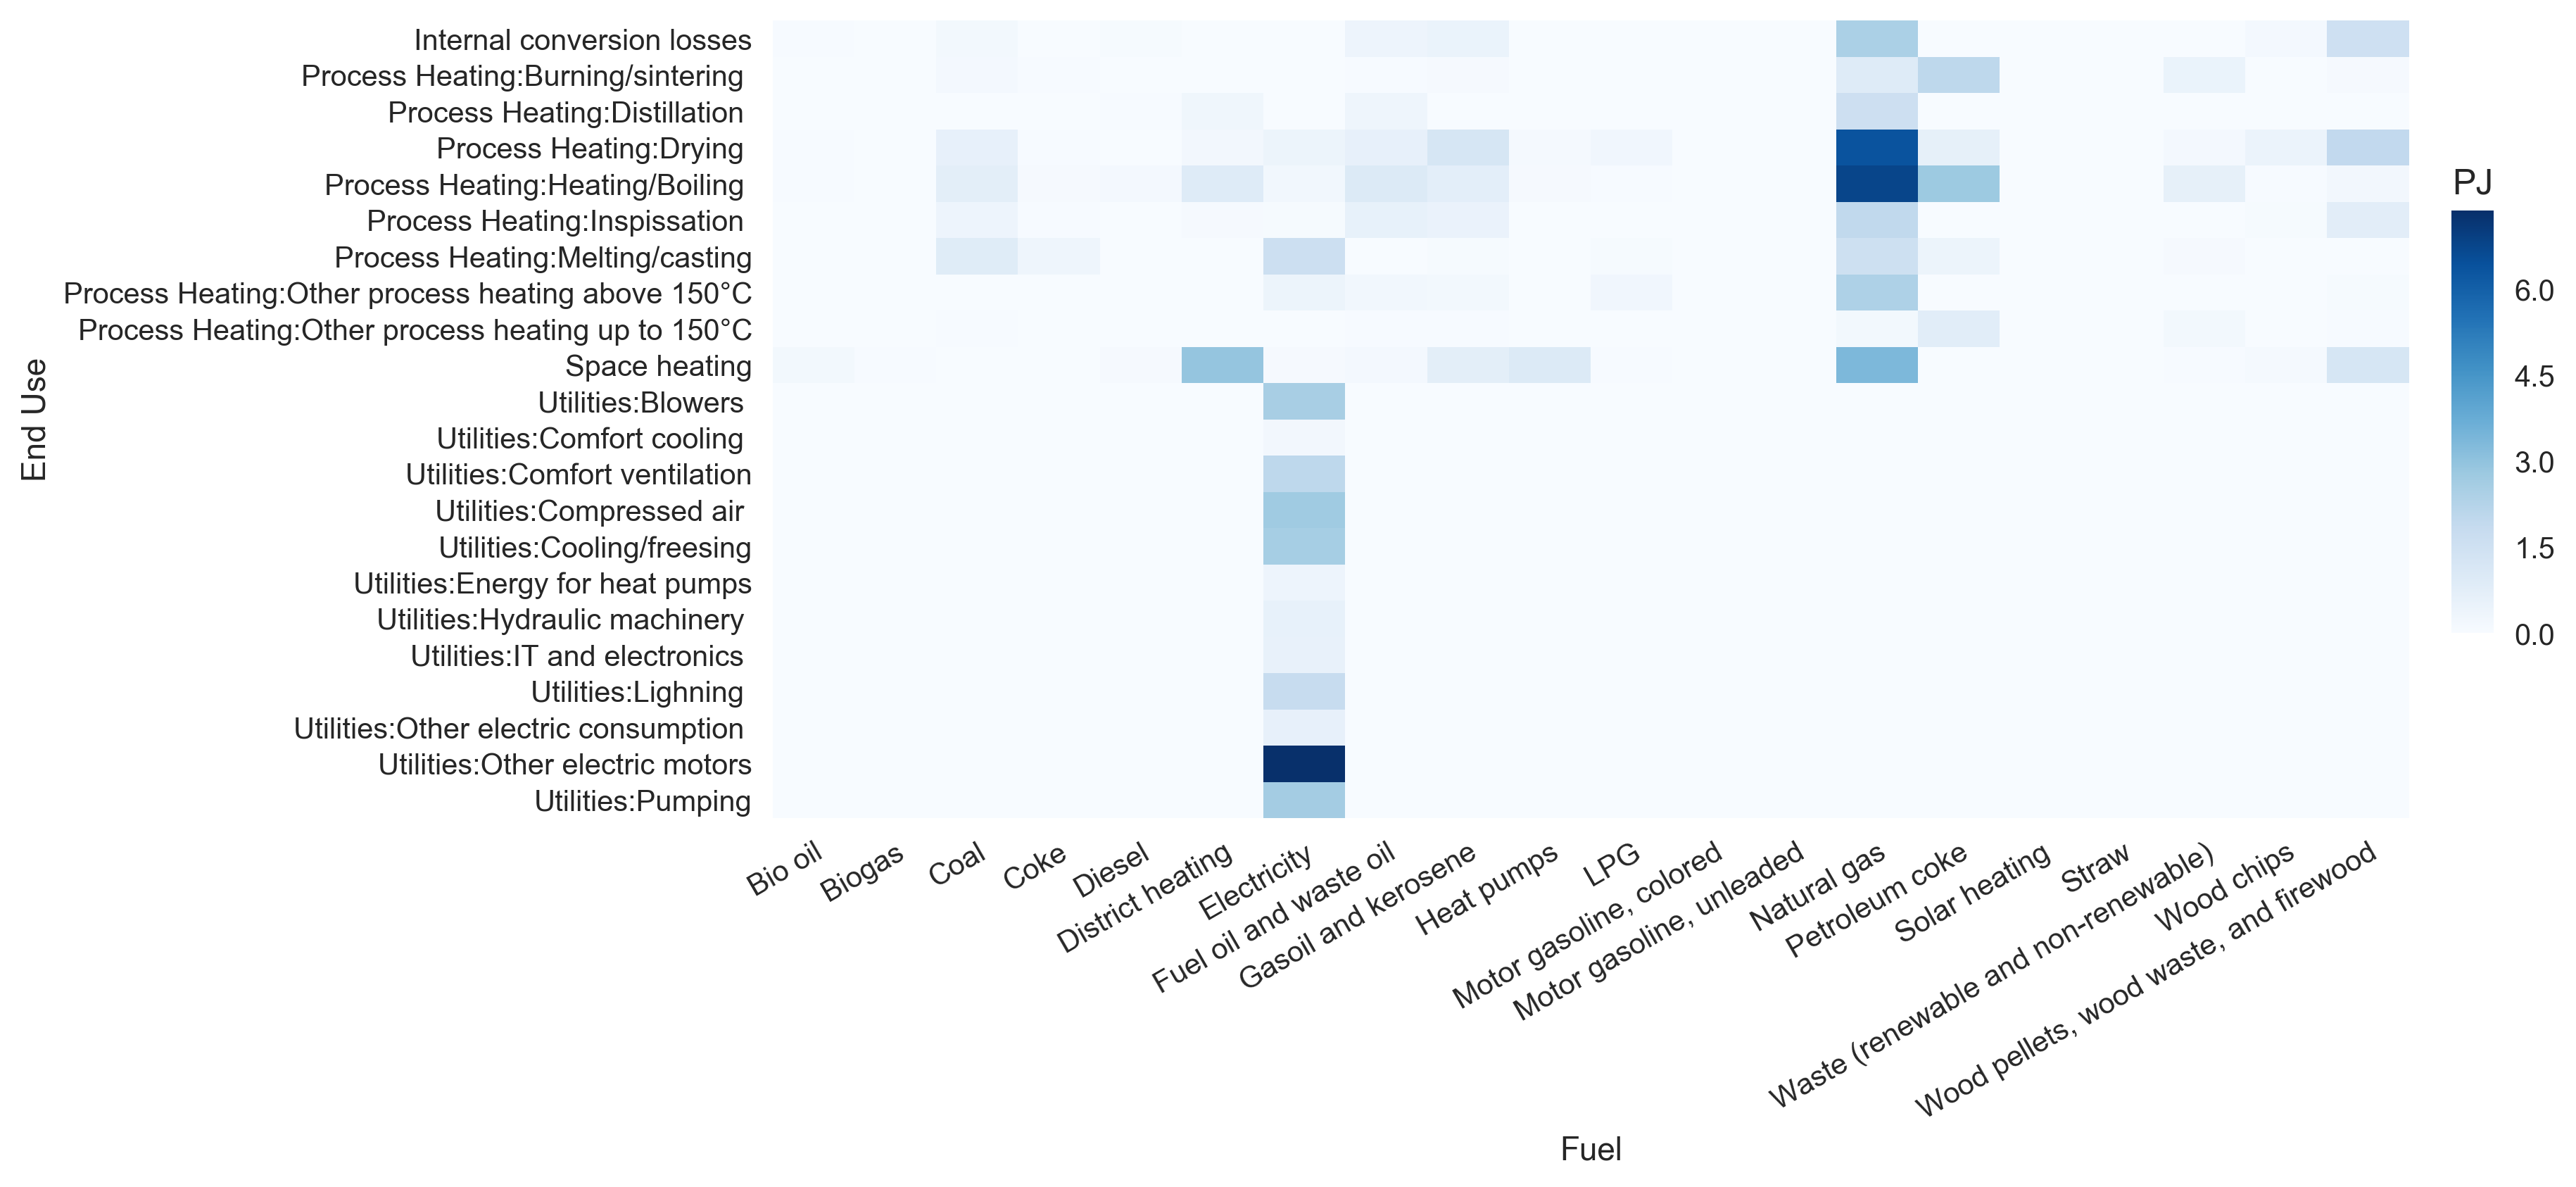
\includegraphics[width=\linewidth]{Img/dan_ind/heatmap_prod.png}
\caption{Breakdown of energy consumption by end-use and fuel in production \cite{VM2015}}
\label{heatmapprod} 
\end{figure}
\fi

\subsection{Future work}
\begin{itemize}
    \item integrate vicinity of DH-network (including costs)
    \item deeper and more detailed
    \item more data for profiles (whole Denmark)
    \item each decarbonisation method requires a deep analysis itself, costs very uncertain
    \item heat pumps are crucial, performance, COP very different, but good basis what we did because can be differentiated
\end{itemize}

%%%%%%%%%%%%%%%%%%%%%%%%%%%%%%%%%%%%%%%%%%%%%%%%%%%%%%%%%%%%%%%%%%%%%%%%%%%%%%%%%%%%%

\section{Conclusion} \label{endofpaper}
% The main conclusions of the study may be presented in a short Conclusions section, which may stand alone or form a subsection of a Discussion or Results and Discussion section.

%%%%%%%%%%%%%%%%%%%%%%%%%%%%%%%%%%%%%%%%%%%%%%



%%%%%%%%%%%%%%%%%%%%%%%%%%%%%%%%%%%%%%%%%%%%%%%%%%%%%%%%%%%%%%%%%%%%%%%%%%%%%%%%%%%%%

\section*{Acknowledgements}
The research has been co-financed by Innovation Fund Denmark under the research project SAVE-E (grant no. 4106-00009B) and the research project FUTURE GAS (grant no. 5160-00006B).
The authors also thank the institutions which gave access to relevant data: the Danish Energy Agency (Energistyrelsen, DEA) and the energy consulting company Viegand Maagøe.
This paper develops on work presented first at the $12^{th}$ SDEWES 17 Conference on sustainable development of energy, water and environment systems at Dubrovnik, Croatia.

%%%%%%%%%%%%%%%%%%%%%%%%%%%%%%%%%%%%%%%%%%%%%%%%%%%%%%%%%%%%%%%%%%%%%%%%%%%%%%%%%%%%%

\section*{Comments for final check}

INTRODUCTION
\begin{itemize}
    \item all needs to be decarbonised, but industry especially difficult and diverse
    \item define industry for our paper
    \item Non-residential energy demand (industry) constitutes a
substantial share of total energy demand
    \begin{itemize}
        \item EU: production and agriculture 28\% / services 13\% \cite{Eurostat2017}
        \item Denmark: production and agriculture 20\% / services 13\% \cite{DanishEnergyAgency2014}
    \end{itemize}
    \item Usage of energy in industry is diverse regarding
        \begin{itemize}
            \item End-use / required type of energy / temperature levels
            \item Fuels
            \item Temporal profiles
            \item Demand flexibility
        \end{itemize}
    \item Solutions and challenges to go 100\% renewable are diverse
    \item Interaction with the rest of the energy system decisive
    \item Thus, it is important to model in detail and in the context of the whole integrated energy system
    \item review on what has been done for industry modelling (method-wise) and what came out (numbers)
    \item explain scope and focus on Denmark?
    \item outline paper: This paper gives 
\end{itemize}

MODELLING
%Provide sufficient details to allow the work to be reproduced by an independent researcher. Methods that are already published should be summarised, and indicated by a reference. If quoting directly from a previously published method, use quotation marks and also cite the source. Any modifications to existing methods should also be described.
Industry plays a decisive part in the integrated energy system. The following energy system analysis questions appear:
\begin{itemize}
    \item Saving potential
    \item Fuel shift potential to gas, renewable gas
    \item Electrification potential
    \item Flexibility potential
    \item Usage of excess heat
    \item Usage of district heating
\end{itemize}
For an integrated modelling approach, a high level of detail required for
\begin{itemize}
    \item Fuel Usage
    \item End-use: electricity, heat specified by temperature levels
    \item Time: Temporal demand profiles
    \item Geography: Vicinity to heat demand / district heat network
    \item Industry group
\end{itemize} 
% \begin{itemize}
%     \item Overview whole model (Balmorel)
%     \item Zoom into industry add on (Figure)
%     \item Describe concept behind industry add on and heat transfer including formulas
%     \item Level of detail: Geographically, technologies, end-use
%     \item Data derivation (Could also be an own section or subsection)
% \end{itemize}

RESULTS
% Results should be clear and concise.
Concluding the numbers. This I know how to calculate:
\begin{itemize}
    \item How much industry already uses district heat?
    \item How much industry already uses heat pumps?
    \item How high is the potential for more industry using district heat?
    \item Which percentage/amount of fossil fuel/installed capacity can be electrified to which cost in which industry group (DGC-data)?
    \item What is the fuel switch options to which cost: Maybe we should have a table with the sectors and end-uses their options to decarbonise.
\end{itemize}
This would be nice to get, but probably only modelling possible:
\begin{itemize}
    \item electricity, process, space heat saved
    \item process, space heat electrified
    \item fuel switched
    \item district heating utilised by industry
    \item excess heat utilised additionally from industry
    \item costs
    \item emissions saved
    \item sensitivities
\end{itemize}

DISCUSSION
% This should explore the significance of the results of the work, not repeat them. A combined Results and Discussion section is often appropriate. Avoid extensive citations and discussion of published literature.
\begin{itemize}
    \item discuss the derived numbers: upper or lower bound, how good can they be? Where do we need to go further?
    \item Which options to decarbonise industry are promising from that numbers? Where do we need to go deeper?
    \item What would be different in other countries? More heavy industry etc.
    \item main other barriers for introducing these that are difficult to capture
    \item policy implications?
    \item further research needs
\end{itemize}



%%%%%%%%%%%%%%%%%%%%%%%%%%%%%%%%%%%%%%%%%%%%%%%%%%%%%%%%%%%%%%%%%%%%%%%%%%%%%%%%%%%%%


%%%%%%%%%%%%%%%%%%%%%%%%%%%%%%%%%%%%%%%%%%%%%%%%%%%%%%%%%%%%%%%%%%%%%%%%%%%%%%%%%%%%%

\section*{References}

\bibliography{mybibfile}

%%%%%%%%%%%%%%%%%%%%%%%%%%%%%%%%%%%%%%%%%%%%%%%%%%%%%%%%%%%%%%%%%%%%%%%%%%%%%%%%%%%%%


\end{document}